\section{Hiện thực hệ thống}
\subsection{Chức năng người dùng}
\subsubsection{Trang chủ}
\begin{figure}[H]
    \centering
    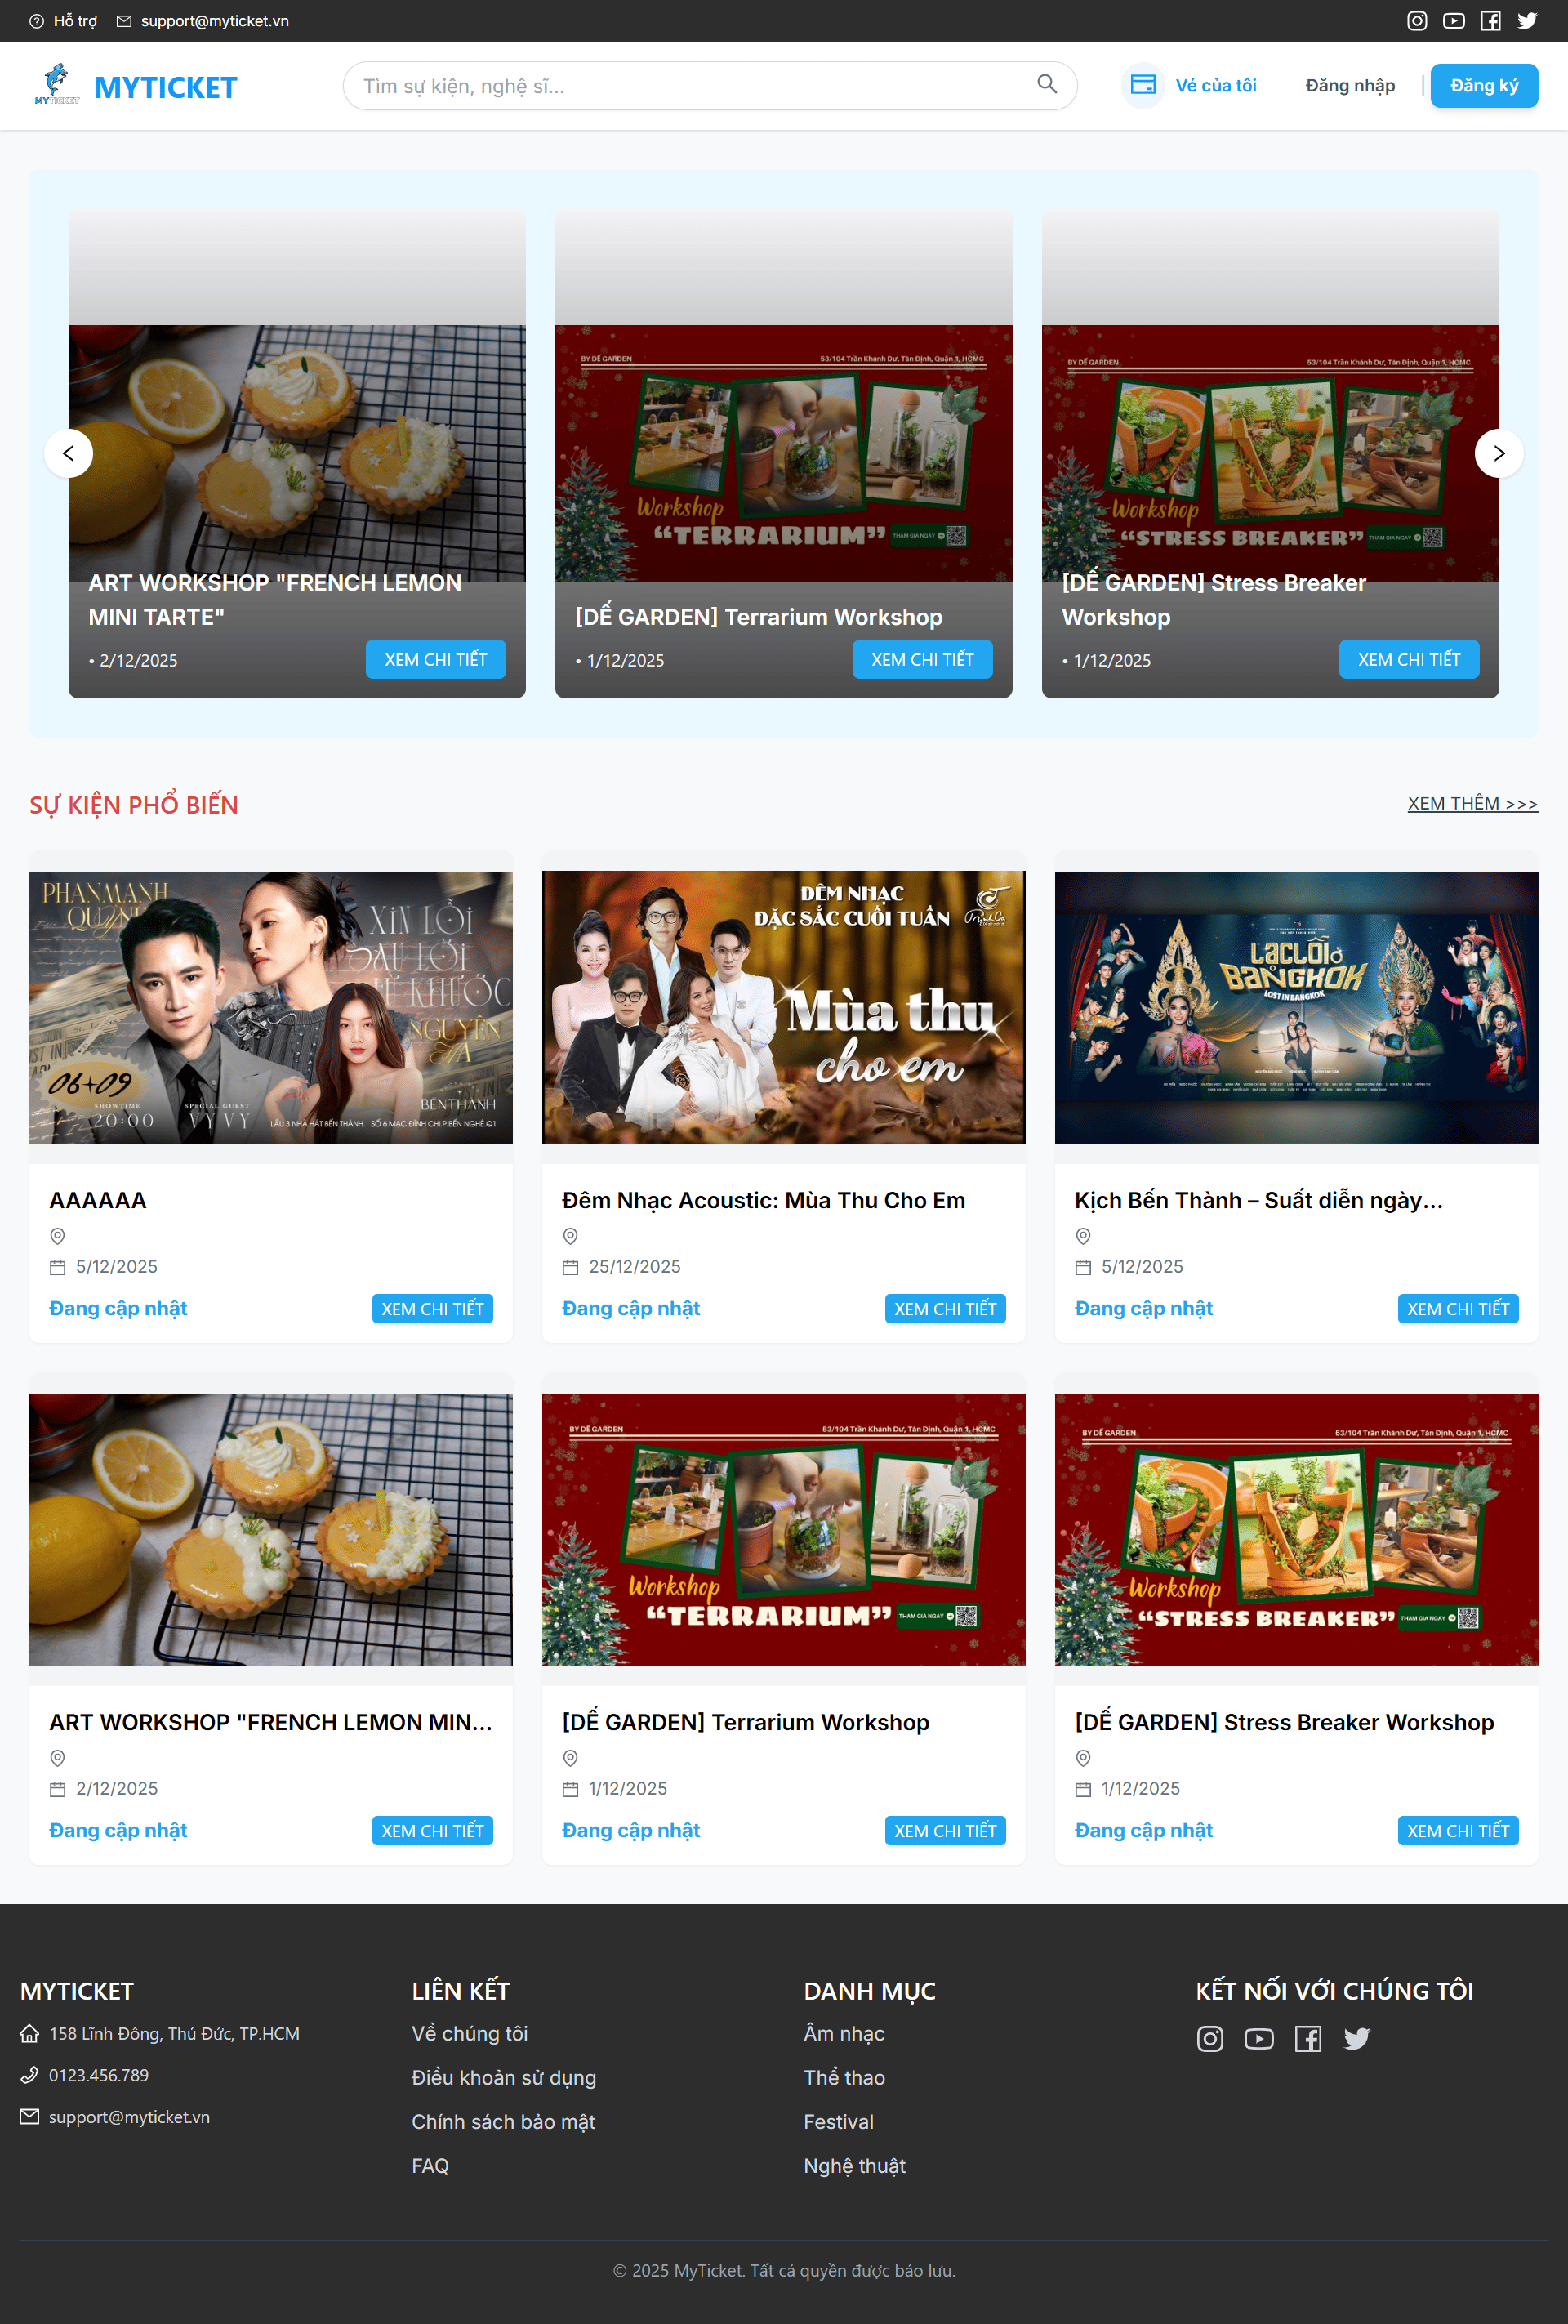
\includegraphics[width=0.75\textwidth]{Contents/UI/USER/Trang chủ.png}
    \vspace{15pt}
    \caption{Giao diện trang chủ}
\end{figure}
\indent \indent Mô tả:\\
\indent - Đây là trang chủ của hệ thống. Trang này hiển thị đanh sách các sự kiện đang được bán vé trong hệ thống với hai mục chính. \\
\indent - Tại đây, người dùng có thể tiến hành xem danh sách các sự kiện, tìm kiếm sự kiện, hỗ trợ chat với quản trị viên hoặc tiến hành đăng nhập hay đăng ký tài khoản.
\subsubsection{Tìm kiếm sự kiện}
\begin{figure}[H]
    \centering
    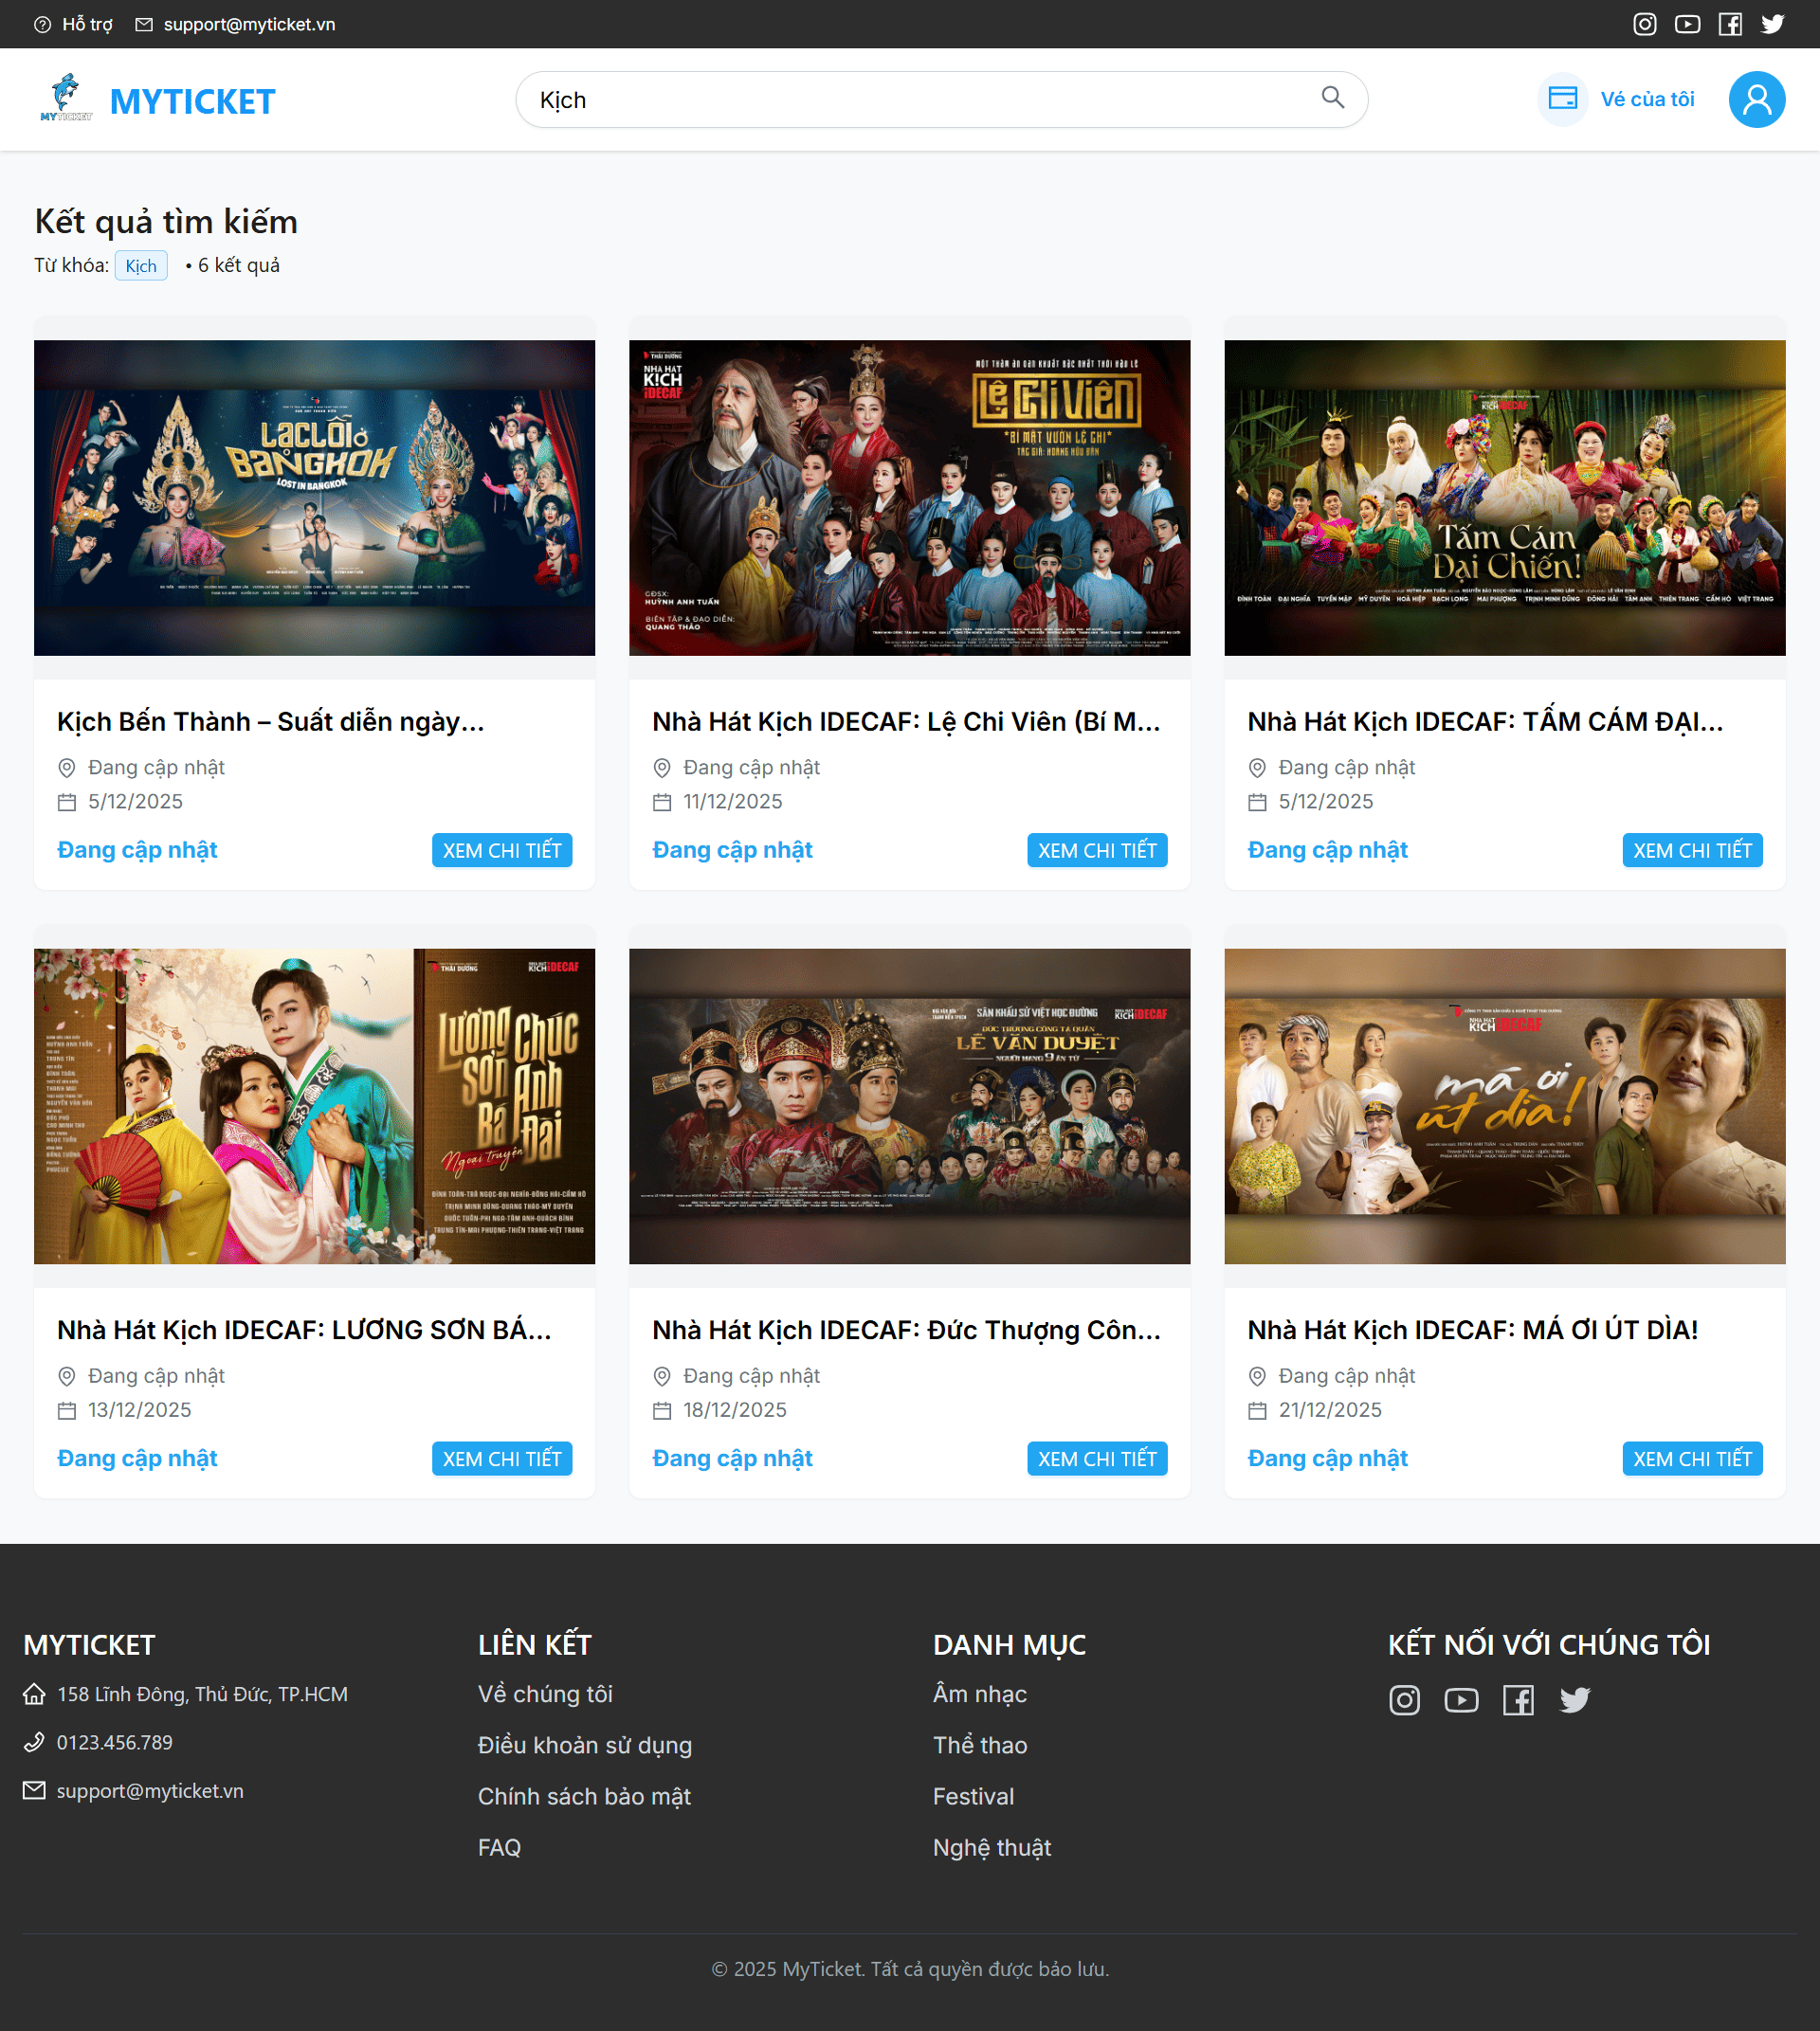
\includegraphics[width=0.75\textwidth]{Contents/UI/USER/kết quả tìm kiếm.png}
    \vspace{15pt}
    \caption{Giao diện kết quả tìm kiếm sự kiện của người dùng khi có sự kiện phù hợp}
\end{figure}
\begin{figure}[H]
    \centering
    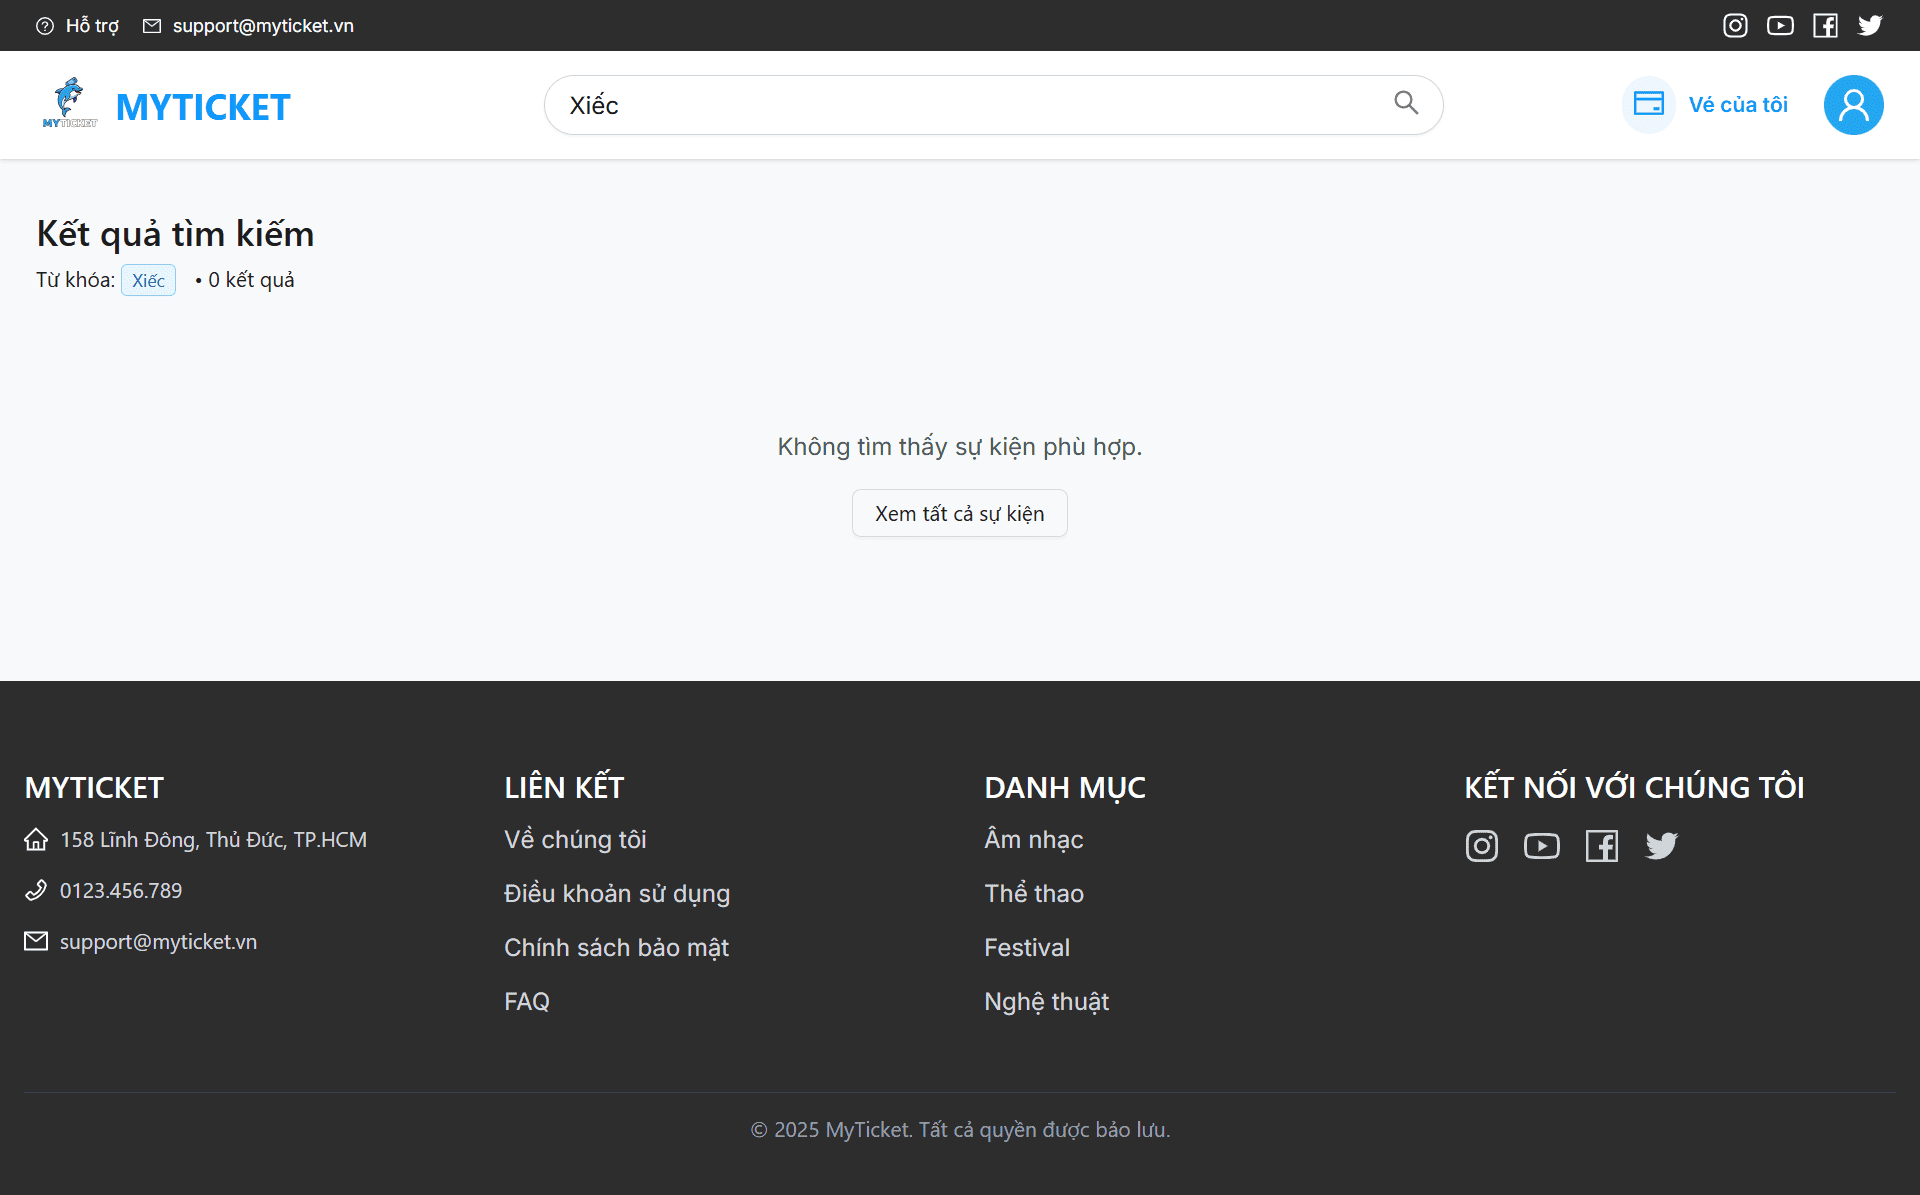
\includegraphics[width=0.75\textwidth]{Contents/UI/USER/tìm kiếm không có kết quả.png}
    \vspace{15pt}
    \caption{Giao diện kết quả tìm kiếm sự kiện của người dùng khi không có sự kiện phù hợp}
\end{figure}
\indent \indent Mô tả:\\
\indent - Khi người dùng nhập từ khóa vào thanh tìm kiếm, hệ thống sẽ truy vấn và trả về các kết quả liên quan.\\
\indent - Trường hợp không có kết quả phù hợp, người dùng có thể chọn xem tất cả sự kiện đang có.
\subsubsection{Đăng nhập/Đăng ký tài khoản}
\begin{figure}[H]
    \centering
    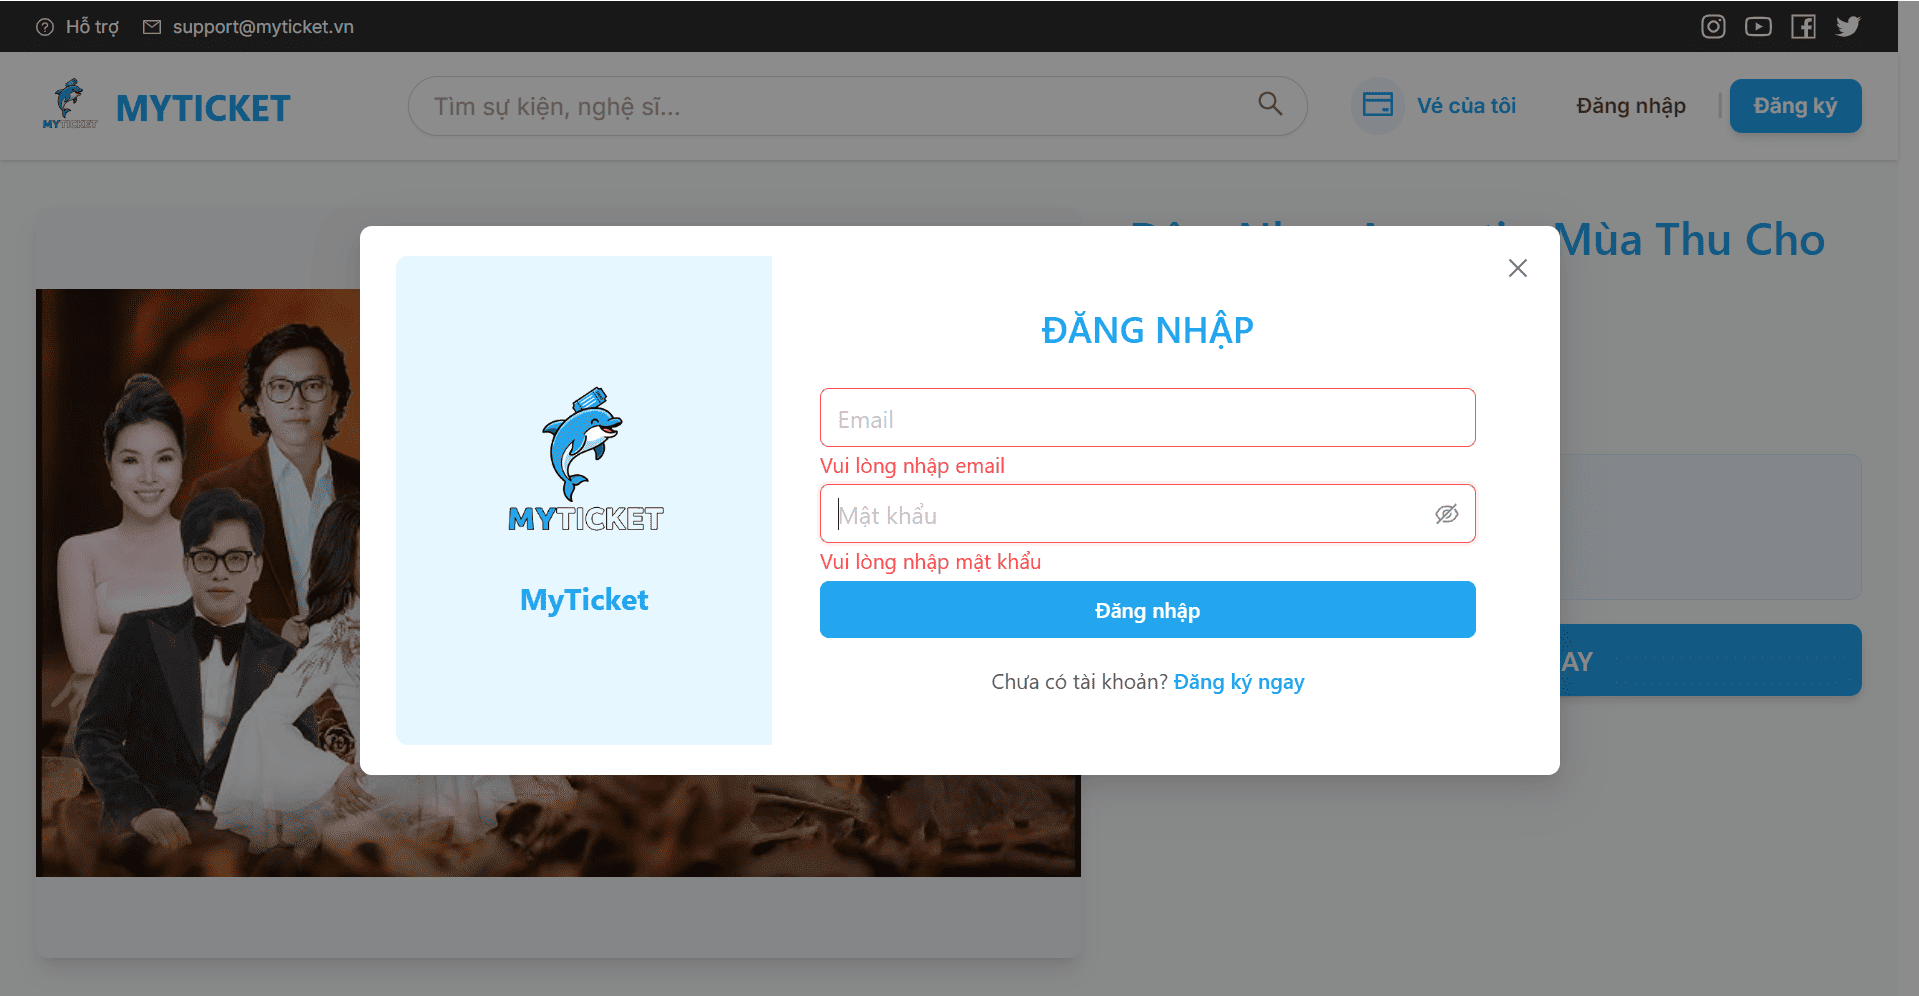
\includegraphics[width=0.75\textwidth]{Contents/UI/USER/Đăng nhập.png}
    \vspace{15pt}
    \caption{Giao diện đăng nhập tài khoản}
\end{figure}
\indent \indent Mô tả:\\
\indent - Người dùng có thể chủ động đăng nhập vào tài khoản bằng cách nhấn vào nút đăng nhập trên thanh Header với hai trường thông được yêu cầu. \\
\indent - Nếu chưa thực hiện việc đăng nhập mà truy cập vào các chức năng bao gồm "Vé của tôi", "Hỗ trợ", "Mua vé" thì hệ thống sẽ tự động hiển thị form đăng nhập yêu cầu người dùng thực hiện.\\
\indent - Hệ thống xác thực thông tin đăng nhập và kiểm tra vai trò (Quản trị viên/Ban tổ chức) để điều hướng giao diện\\
\indent - Trường hợp chọn chưa có tài khoản, người dùng chọn "Đăng ký ngay" sẽ được điều hướng trang Đăng ký bên dưới. Để tạo tài khoản thành công, người dùng bắt buộc phải điền đầy đủ thông tin ở các trường với đúng format quy định.
\begin{figure}[H]
    \centering
    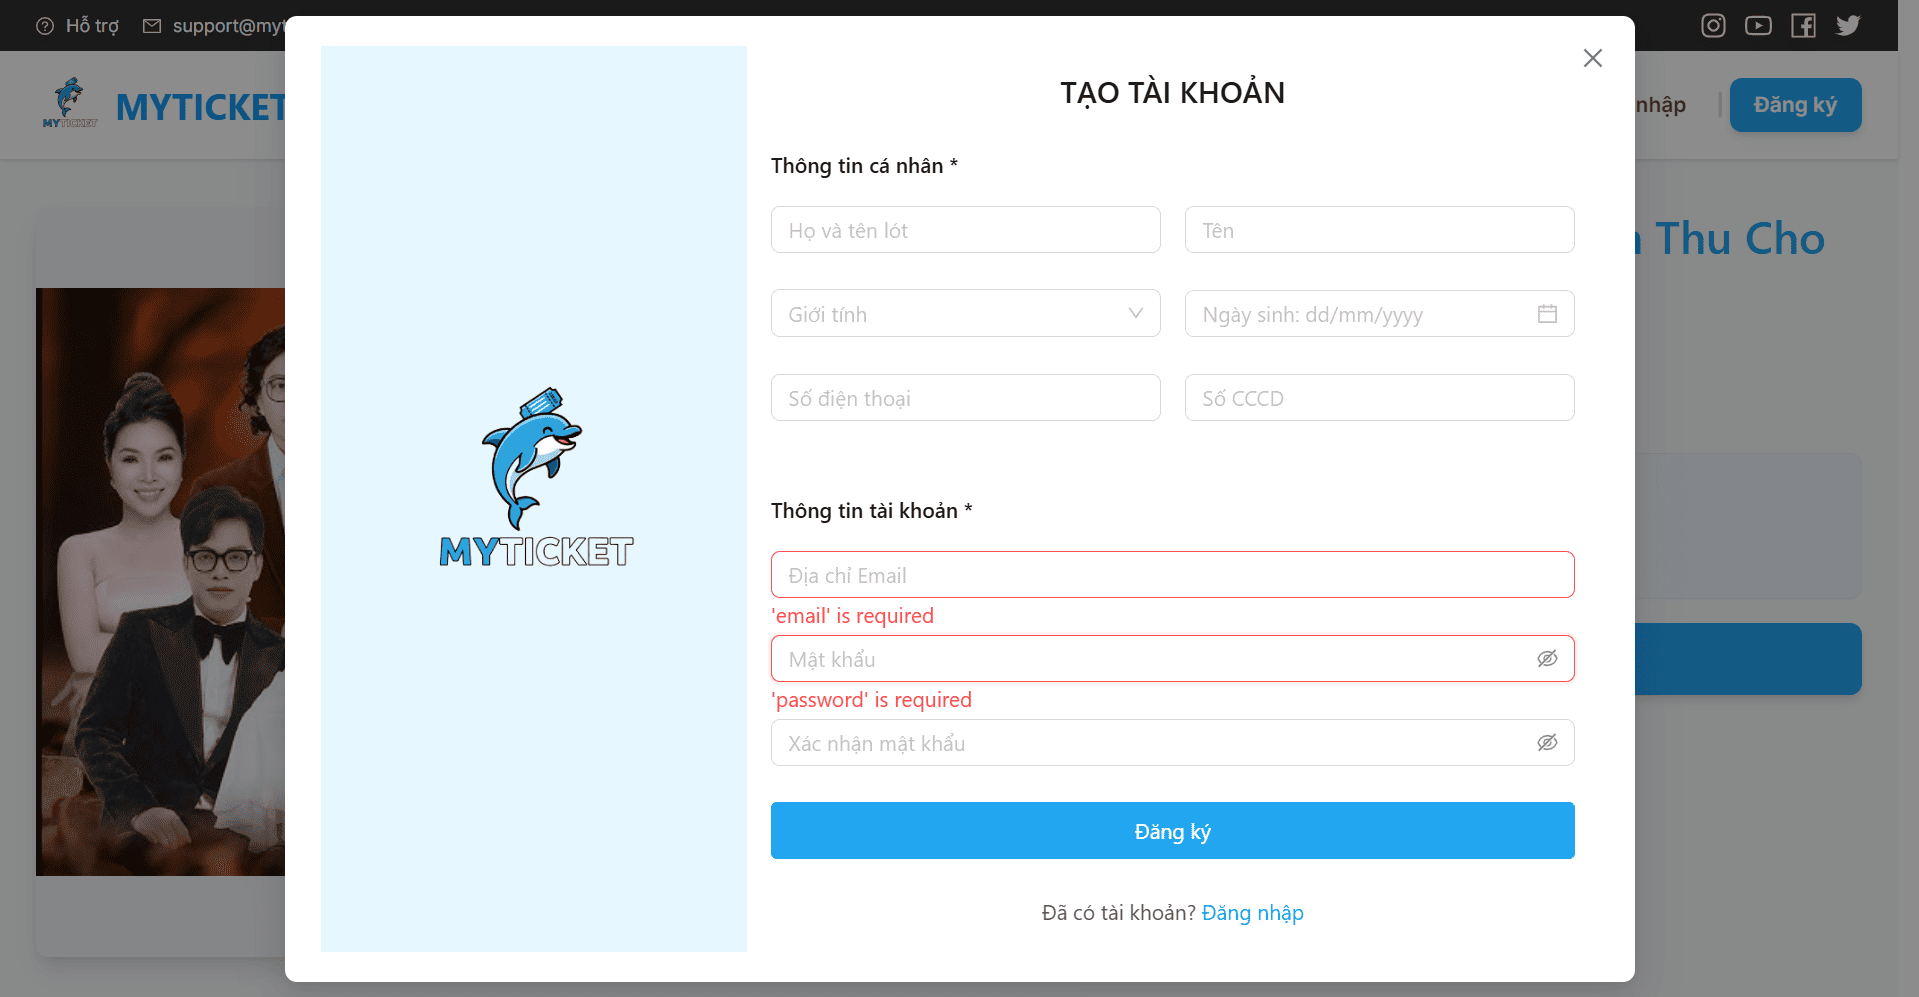
\includegraphics[width=0.74\textwidth]{Contents/UI/USER/Đăng ký tài khoản.png}
    \vspace{15pt}
    \caption{Giao diện đăng ký tài khoản}
\end{figure}
\vspace{-20pt}
\subsubsection{Xem chi tiết thông tin sự kiện}
\begin{figure}[H]
    \centering
    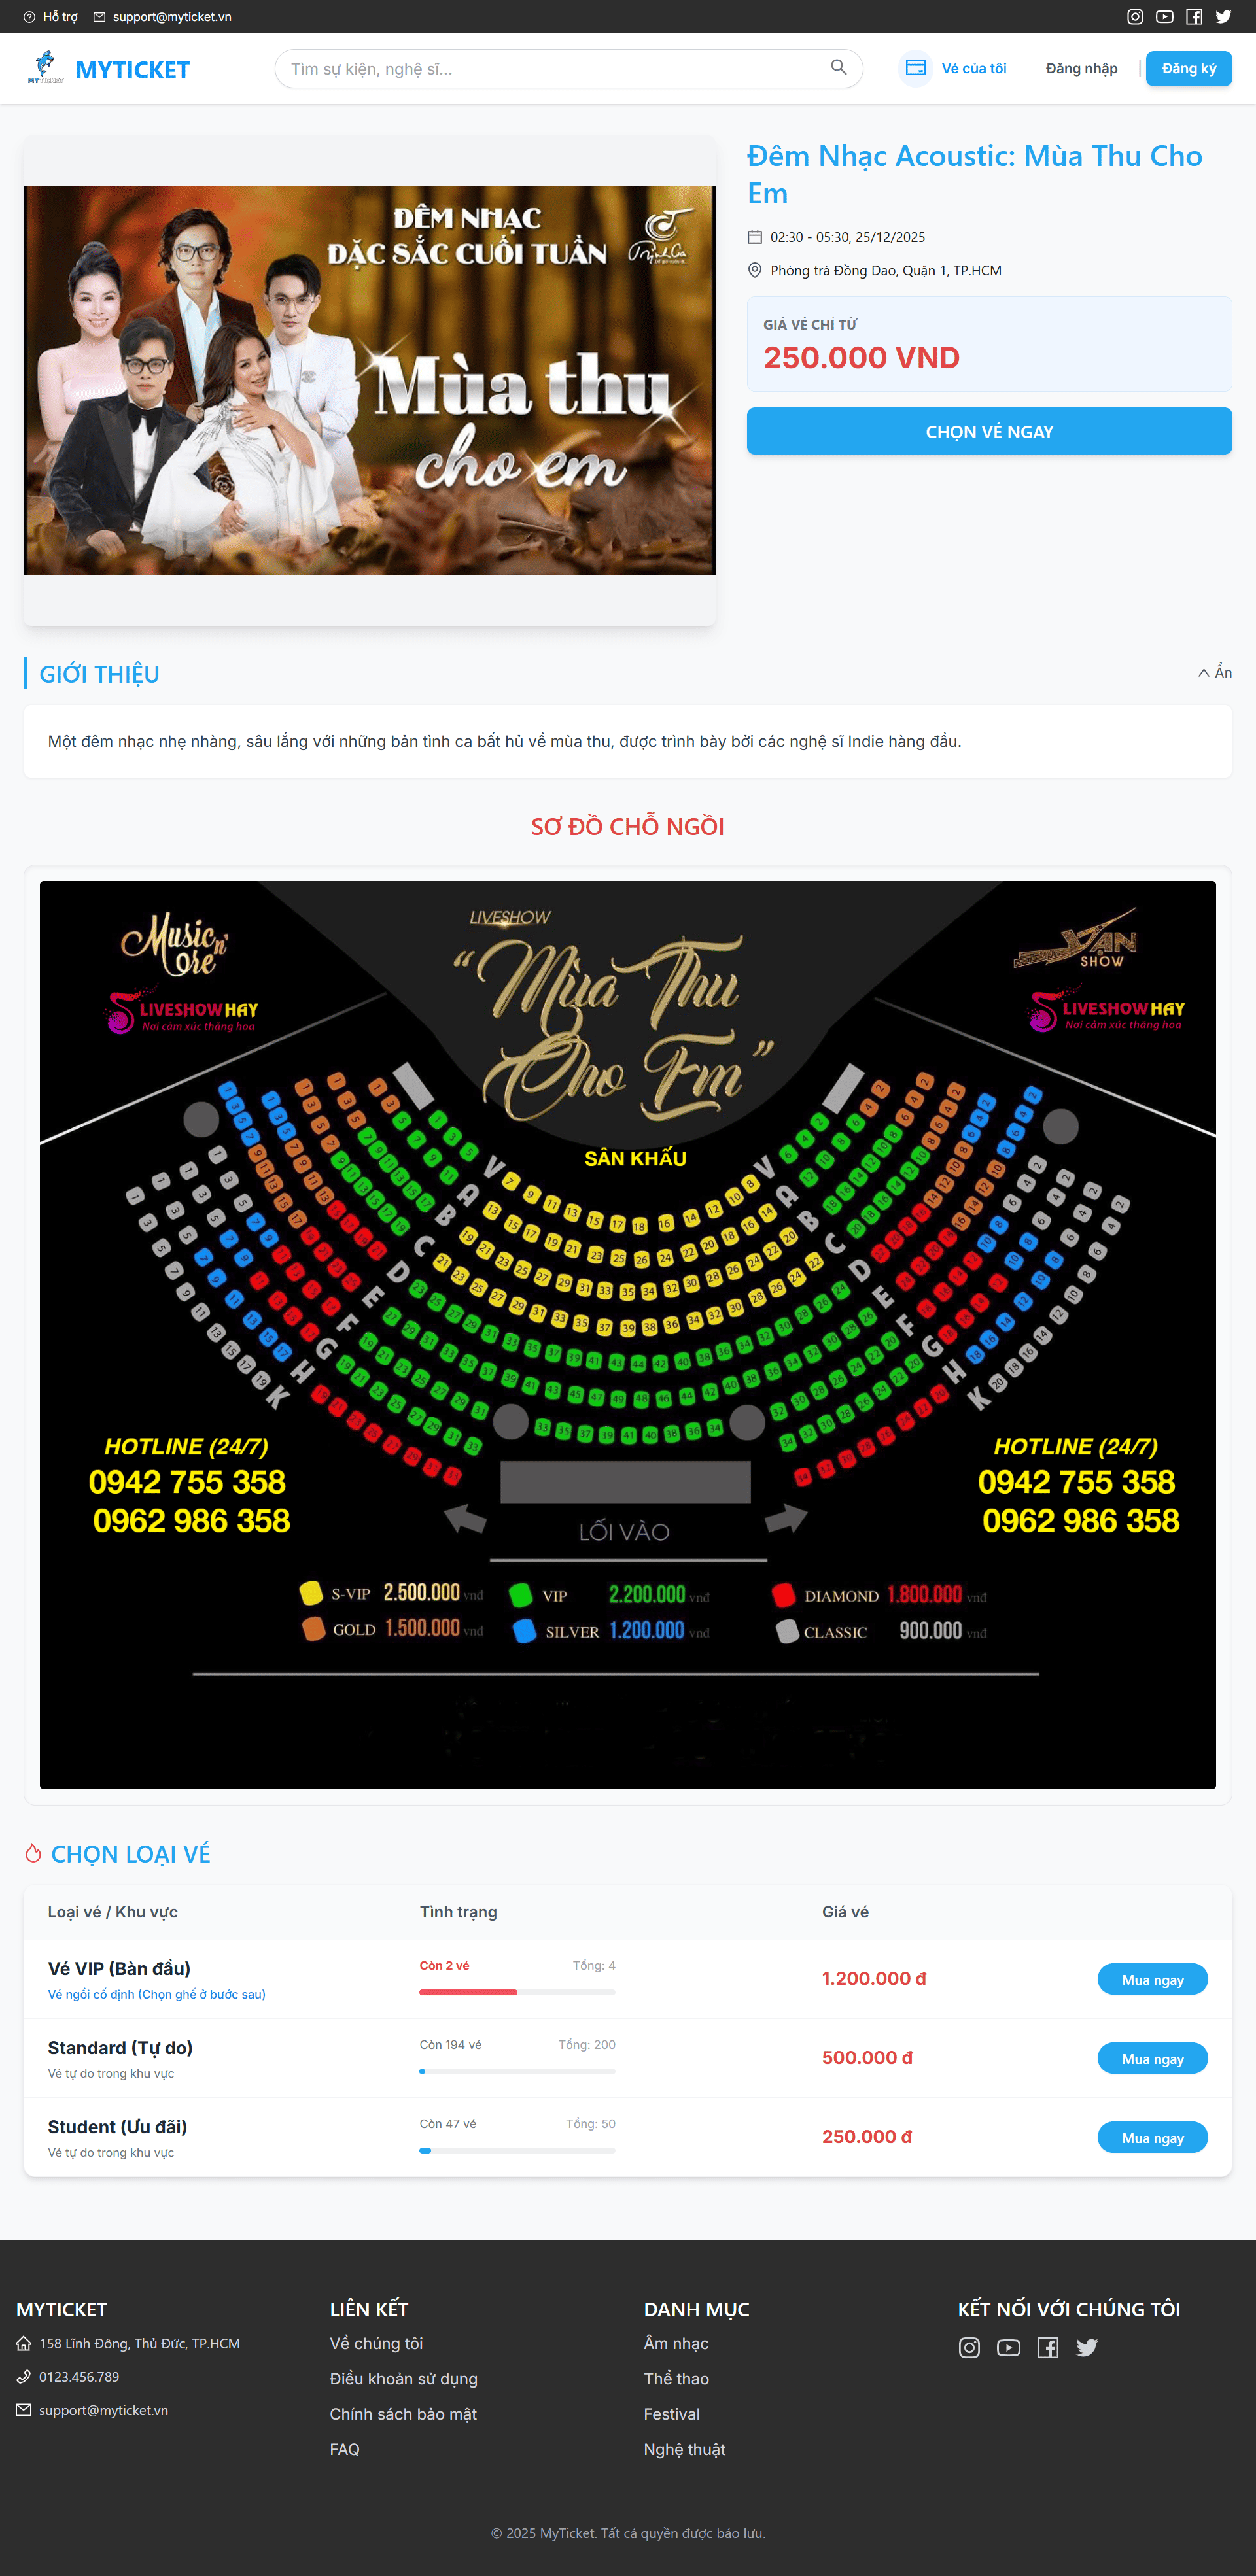
\includegraphics[width=0.70\textwidth]{Contents/UI/USER/Thông tin sự kiện.png}
    \vspace{15pt}
    \caption{Giao diện hiển thị chi tiết thông tin sự kiện}
\end{figure}
\indent \indent Mô tả:\\
\indent - Sau khi nhấn vào nút "Xem chi tiết" của 1 sự kiện cụ thể ở trang chủ, người dùng sẽ được điều hướng đến trang này.\\
\indent - Tại đây, người dùng có thể xem chi tiết thông tin của 1 sự kiện như địa điểm, thời gian tổ chức, mô tả, sơ đồ chỗ ngồi, bảng vé. \\
\indent - Nếu muốn mua vé, người dùng sẽ nhấn vào nút "Mua ngay" của một loại vé cụ thể trong bảng vé. Nếu loại vé nào đã bán hết, nút "Mua ngay" của nó sẽ bị vô hiệu hóa.
\subsubsection{Xác nhận thanh toán}
\begin{figure}[H]
    \centering
    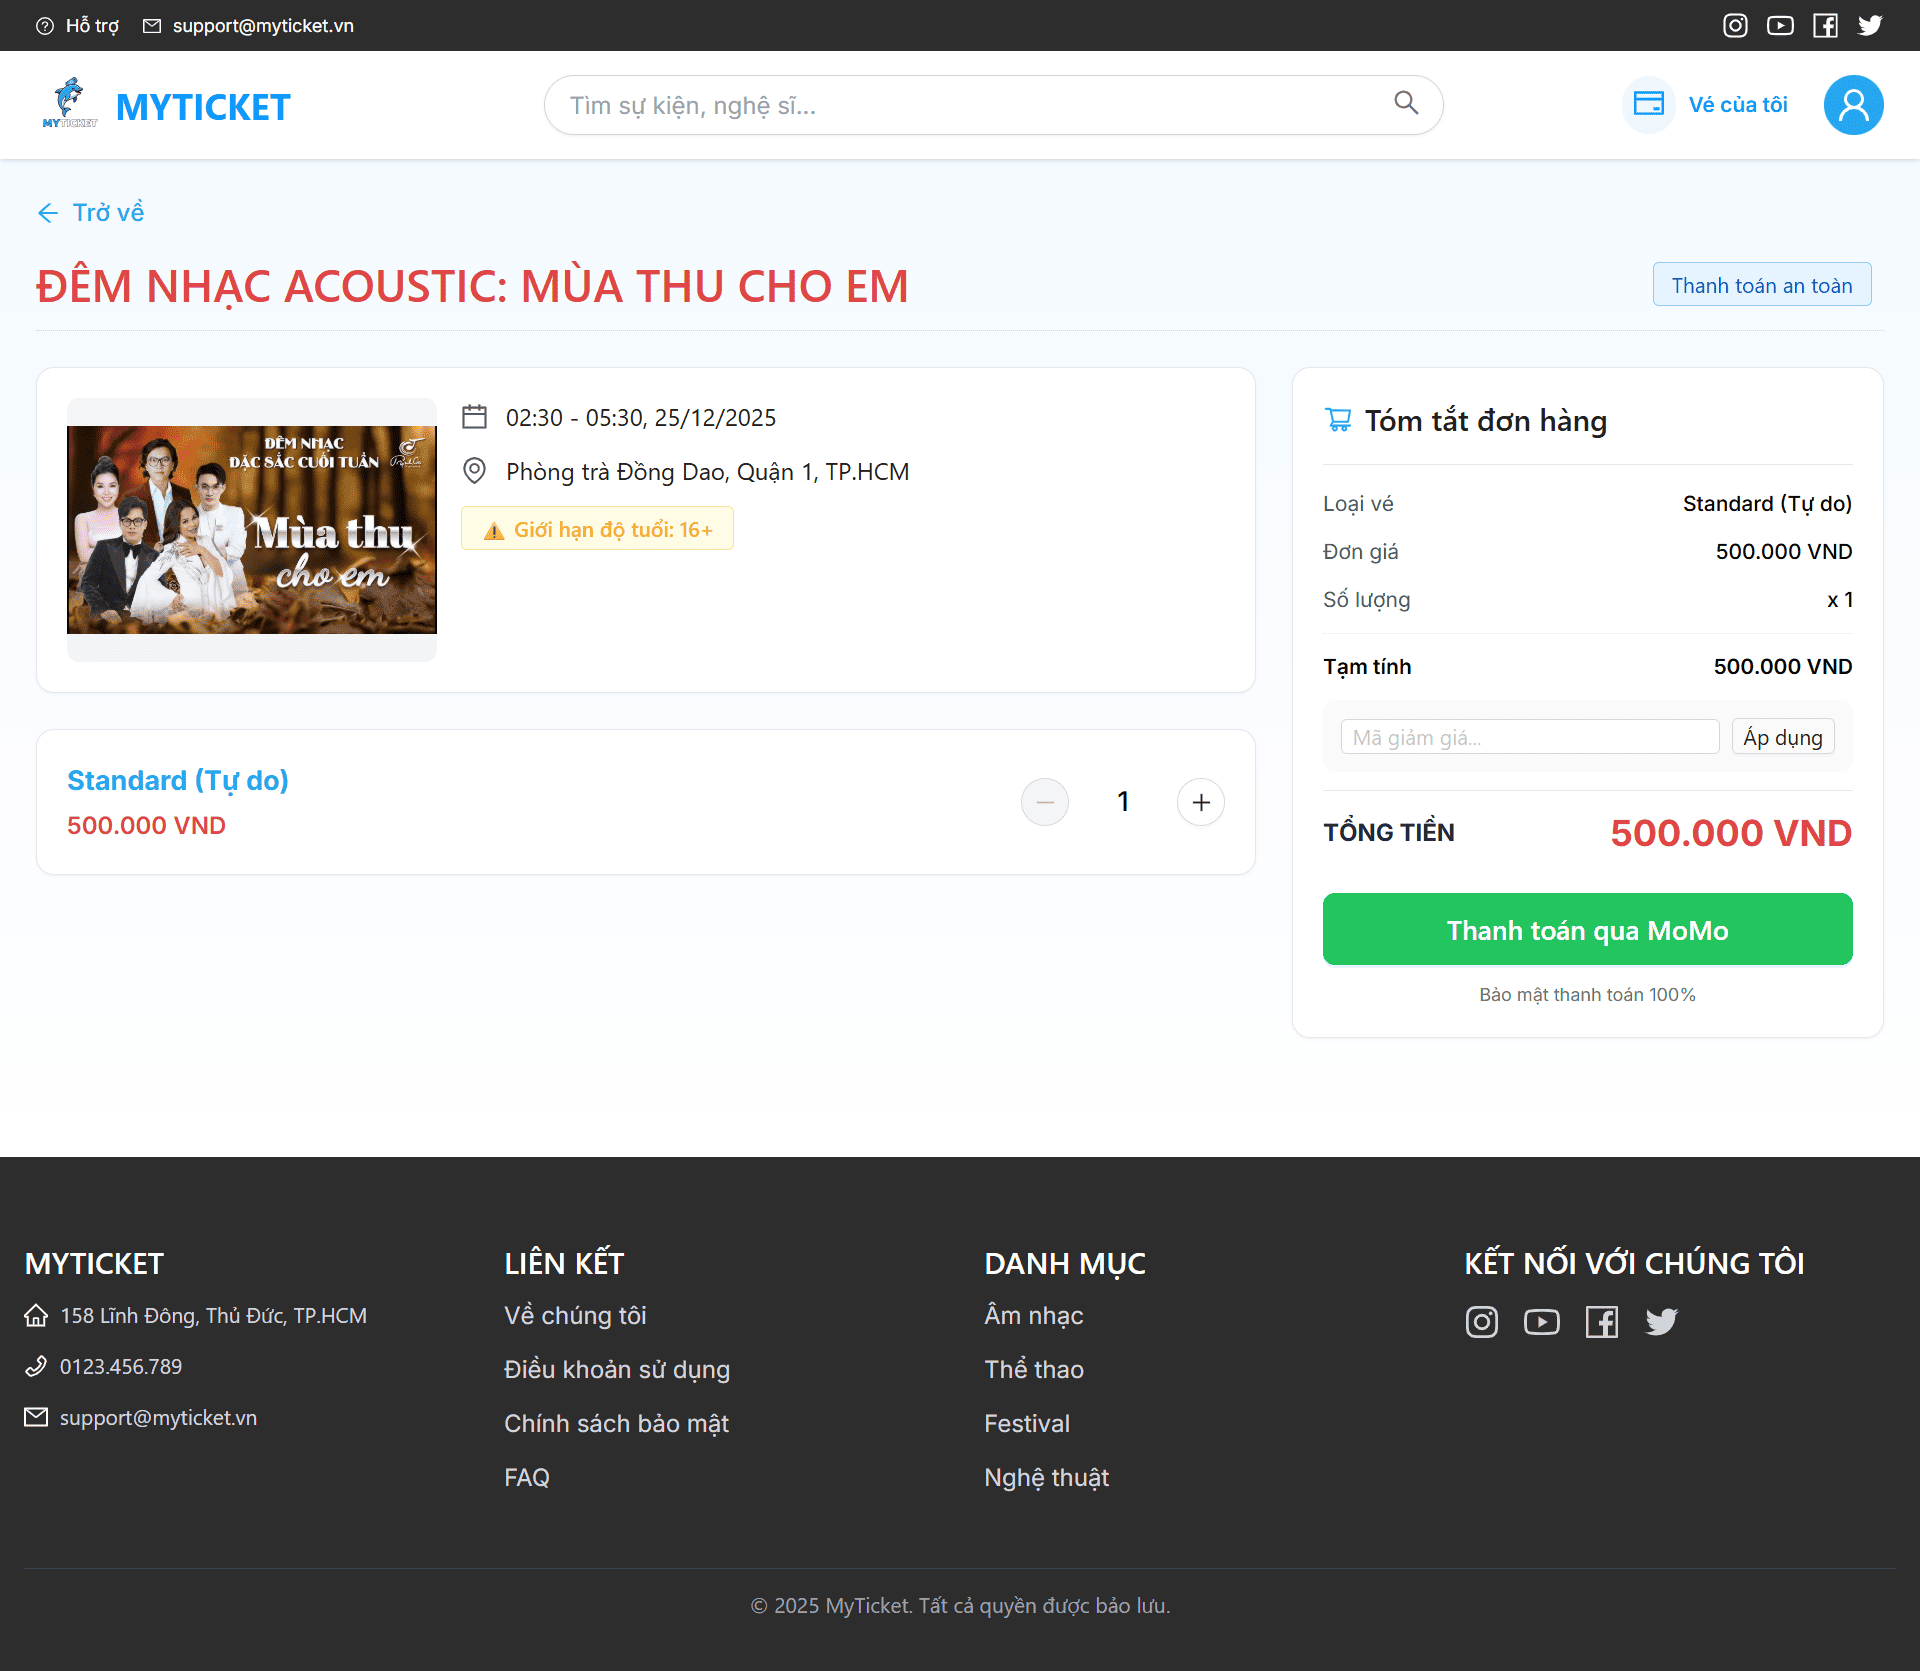
\includegraphics[width=0.75\textwidth]{Contents/UI/USER/Xác nhận thanh toán.png}
    \vspace{15pt}
    \caption{Giao diện xác nhận thanh toán vé sự kiện}
\end{figure}
\indent \indent Mô tả:\\
\indent - Khi chọn mua vé, người dùng sẽ được điều hướng sang trang thanh toán. \\
\indent - Tại đây, người dùng xem được các thông tin liên quan tới vé bao gồm thời gian tổ chức, địa điểm, cảnh báo độ tuổi nếu có, loại vé, số lượng, tổng giá tiền.\\
\indent - Người dùng có thể điều chỉnh số lượng vé muốn mua tùy thích miễn là có đủ số vé. \\
\indent - Đối với loại vé có chỗ ngồi cố định, người dùng được yêu cầu phải chọn thêm vị trí ghế.\\
\indent - Đối với sự kiện có cảnh báo độ tuổi, người dùng sẽ được nhận 1 cảnh báo khi chọn nút "Xác nhận thanh toán" và phải xác nhận mới được tiến hành thanh toán.
\begin{figure}[H]
    \centering
    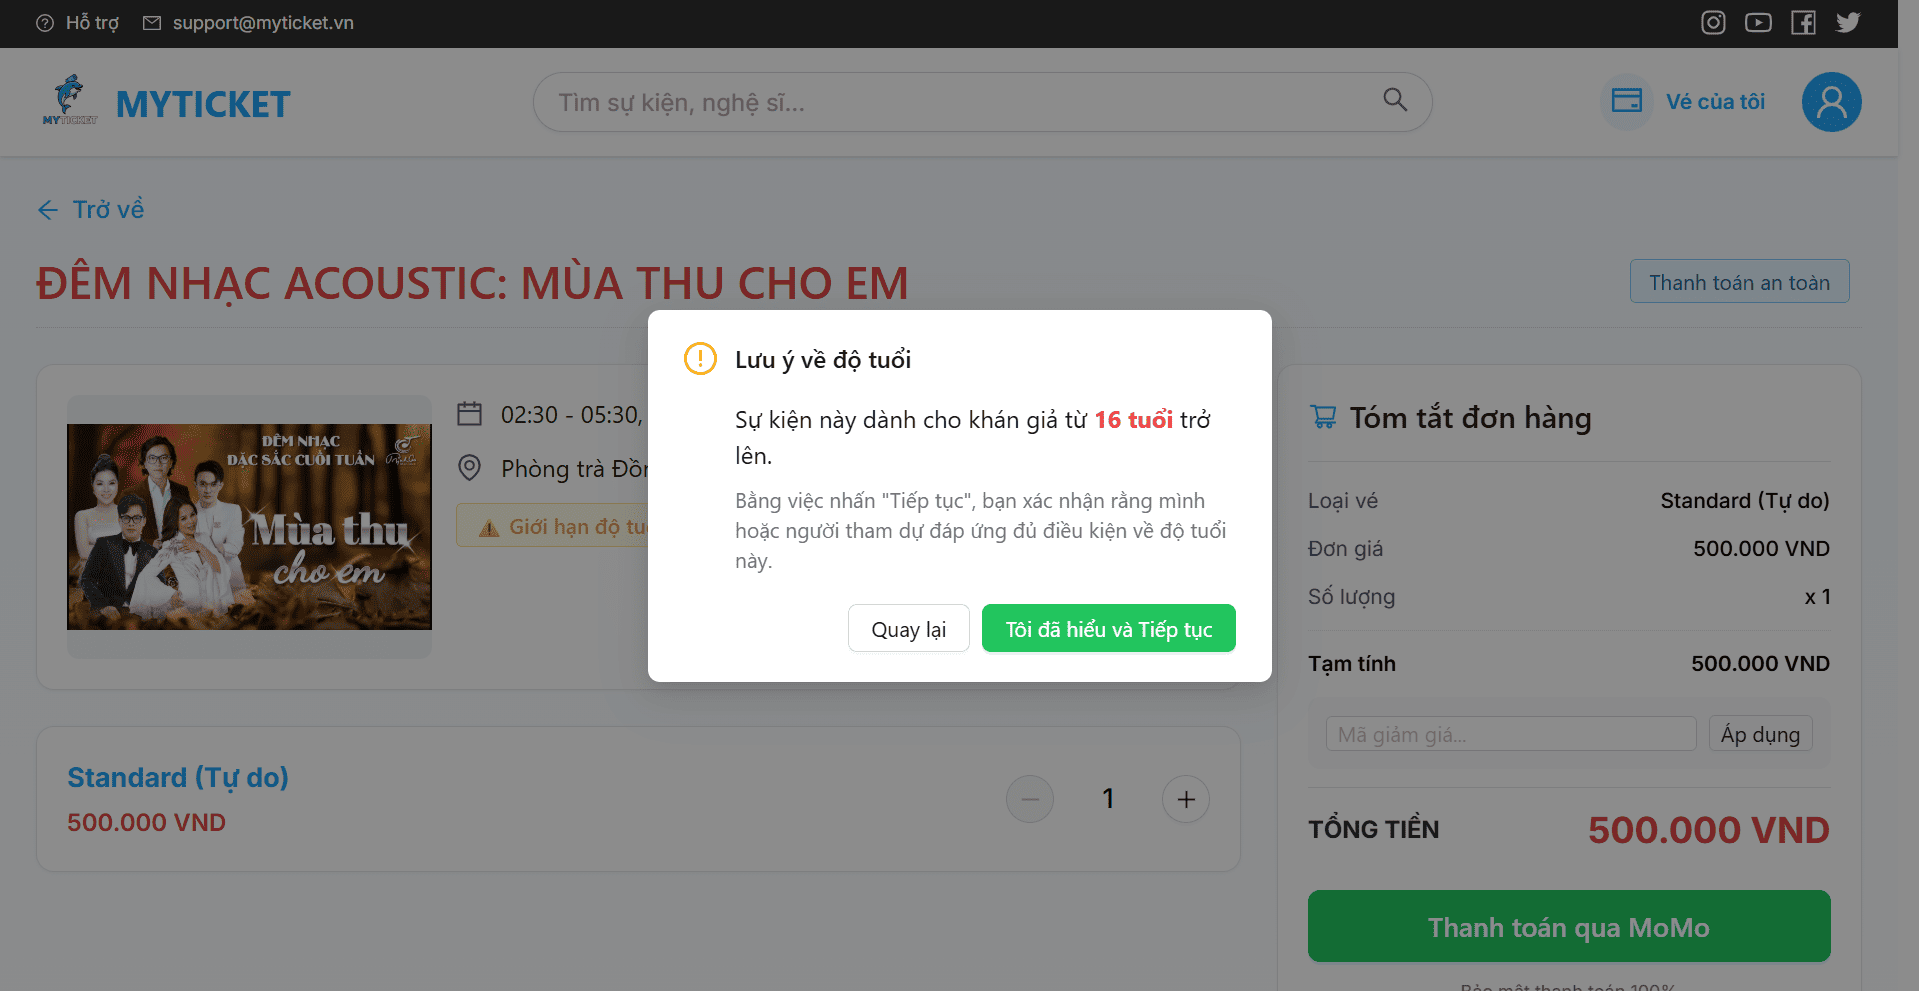
\includegraphics[width=0.75\textwidth]{Contents/UI/USER/Cảnh báo độ tuổi.png}
    \vspace{15pt}
    \caption{Khung tin nhắn cảnh báo độ tuổi}
\end{figure}
\subsubsection{Tiến hành thanh toán}
\begin{figure}[H]
    \centering
    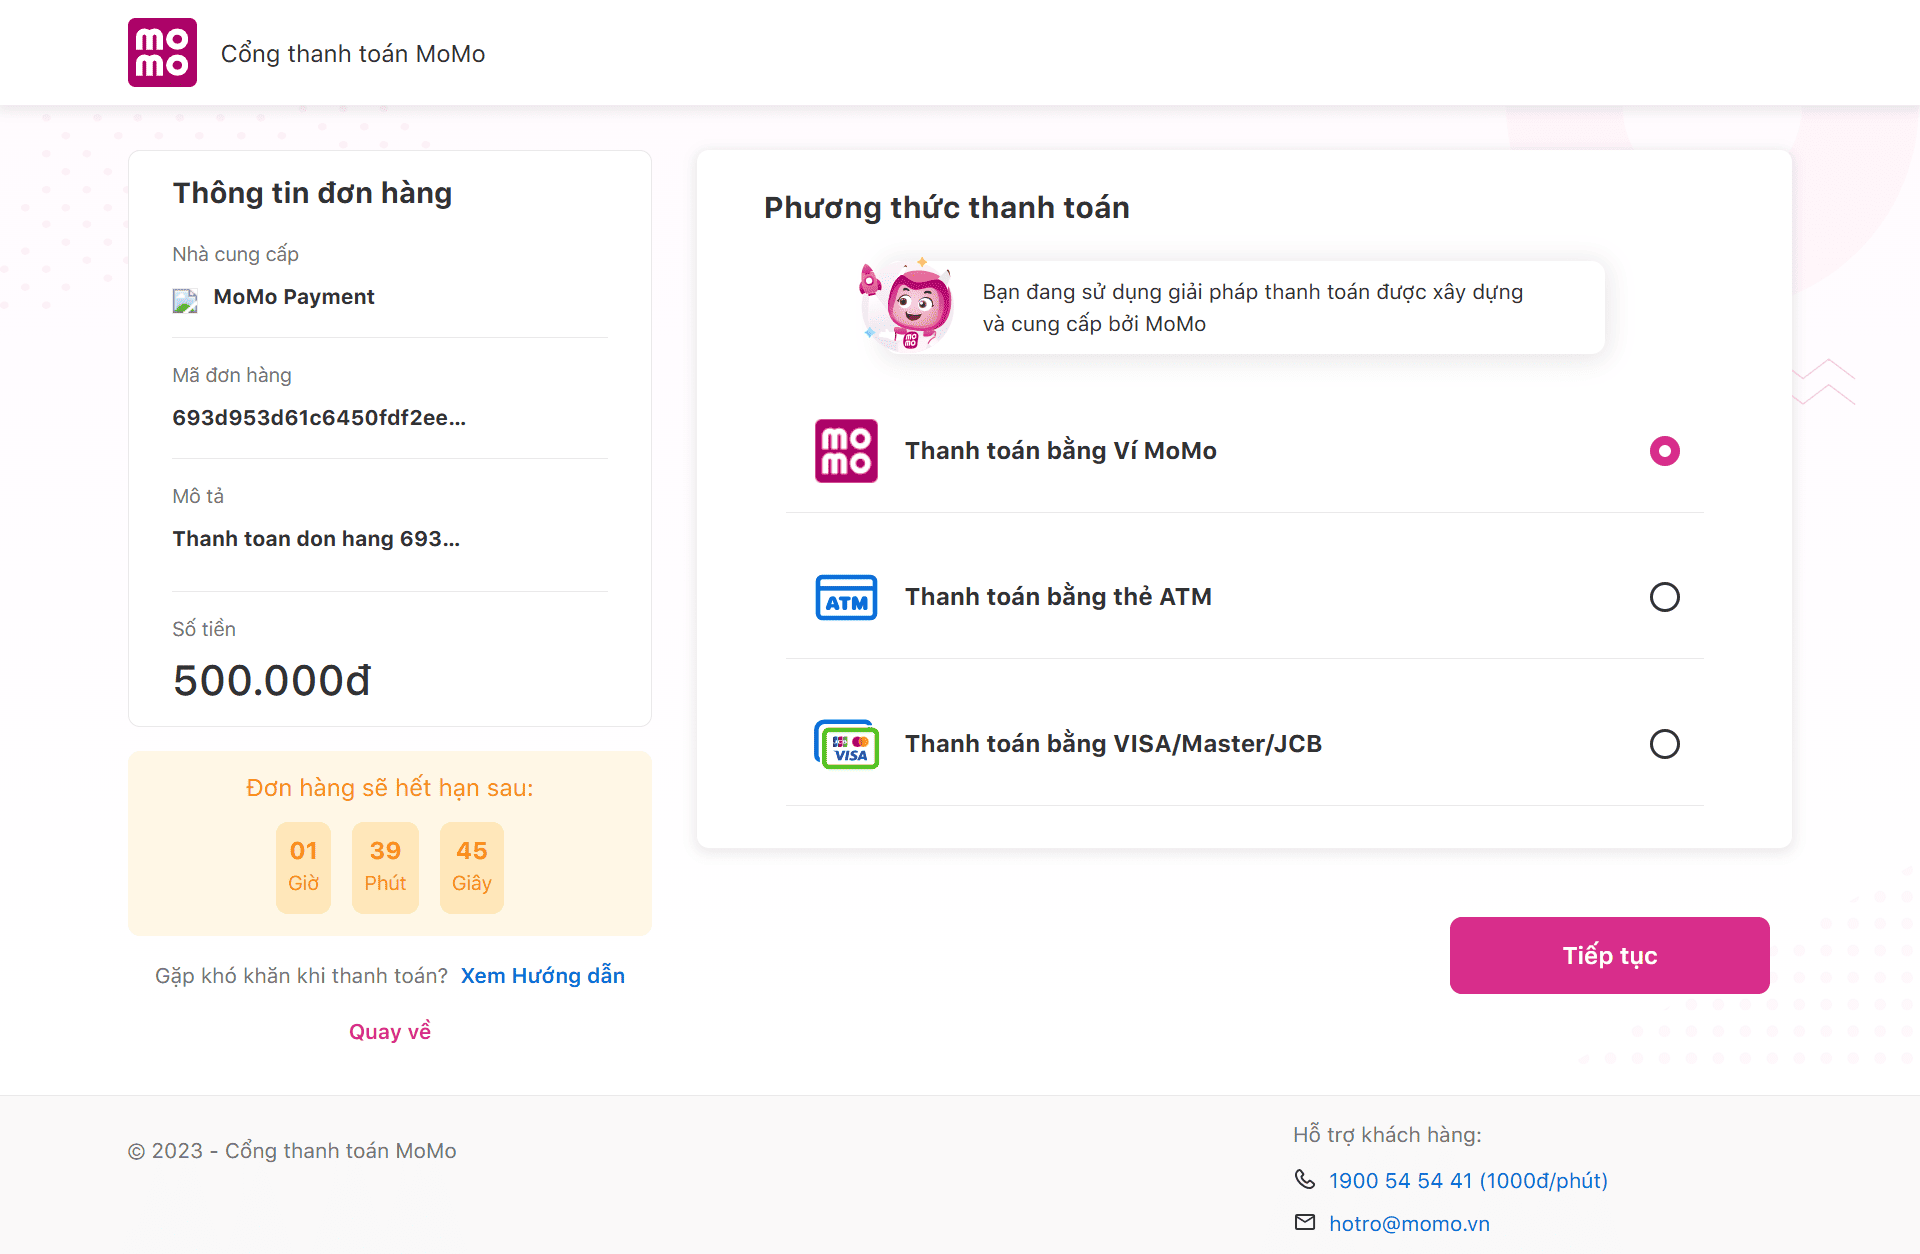
\includegraphics[width=0.75\textwidth]{Contents/UI/USER/Giao diện thanh toán momo.png}
    \vspace{15pt}
    \caption{Giao diện thanh toán liên kết với Momo}
\end{figure}
\indent \indent Mô tả:\\
\indent - Đây là bước cuối cùng để người dùng có thể mua vé thành công. \\
\indent - Chức năng thanh toán của hệ thống được liên kết với nền tảng Momo. Người dùng cần chọn phương thức thanh toán phù hợp và nhập thông liên quan.
\subsubsection{Lịch sử mua vé}
\begin{figure}[H]
    \centering
    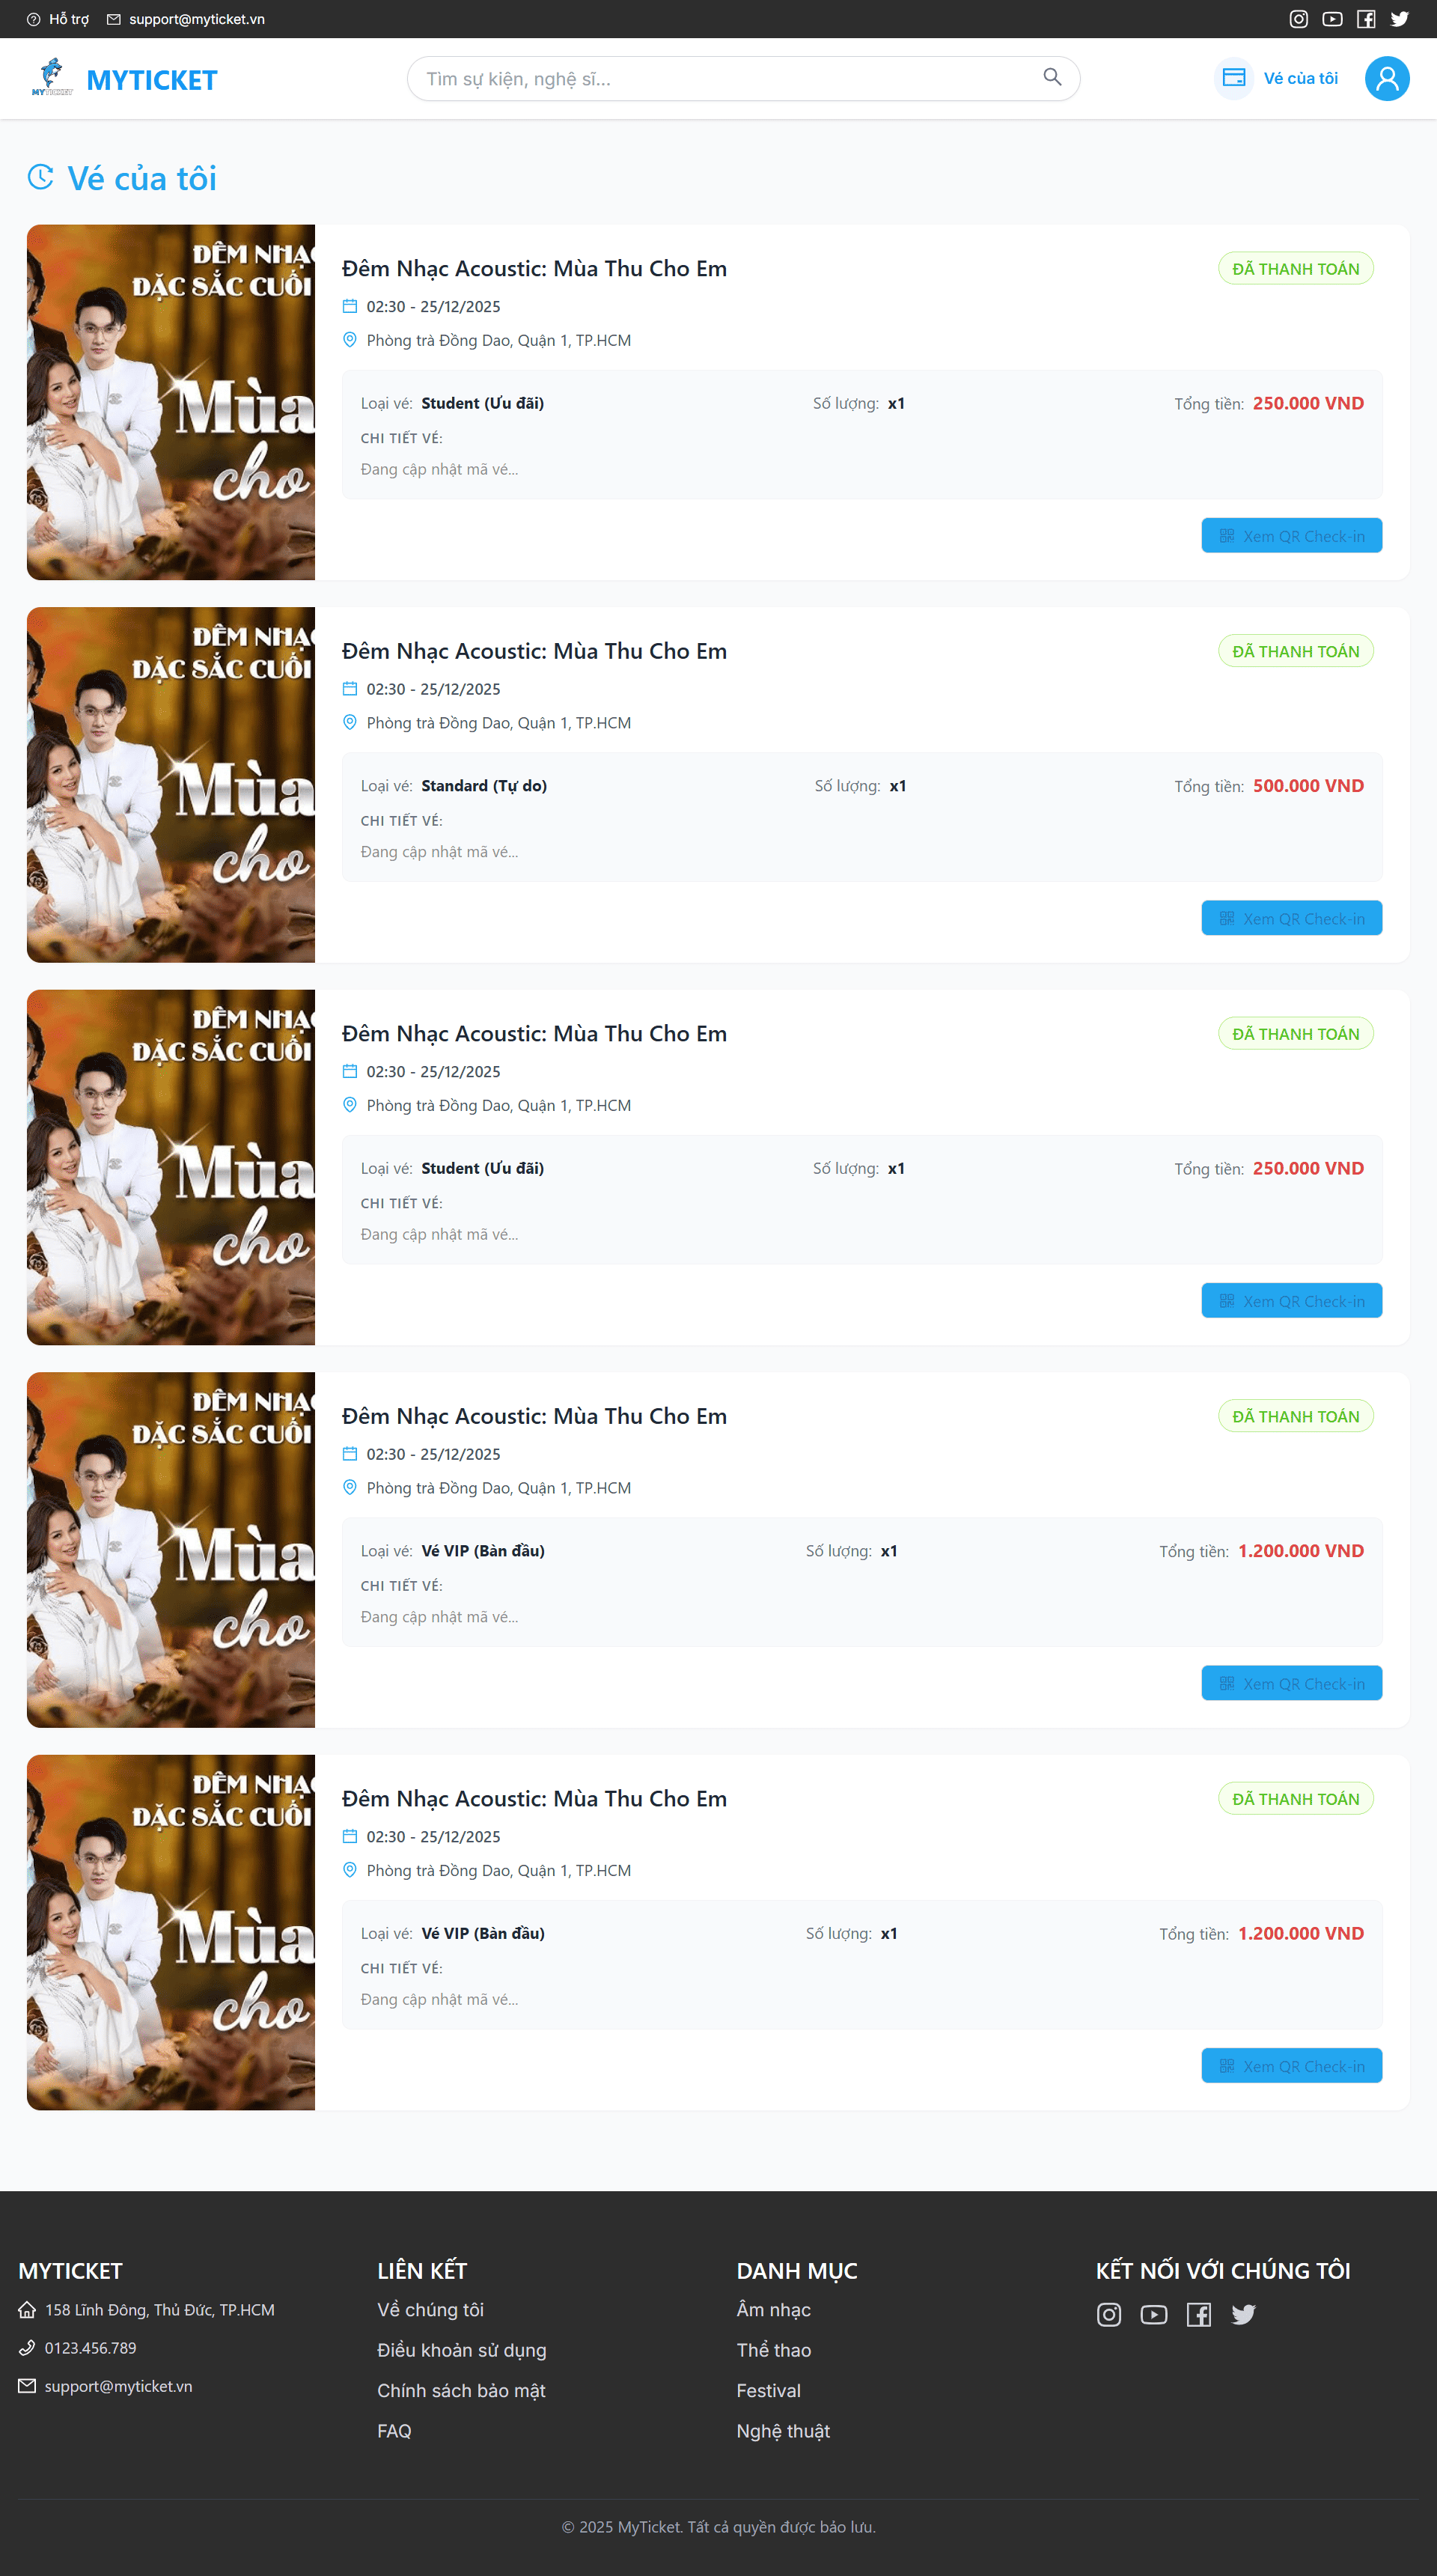
\includegraphics[width=0.75\textwidth]{Contents/UI/USER/Vé của tôi.png}
    \vspace{15pt}
    \caption{Giao diện lịch sử mua vé}
\end{figure}
\indent \indent Mô tả:\\
\indent - Sau khi người dùng mua vé thành công, vé sẽ được lưu và hệ thống tự động điều hướng người dùng đến trang này để xem thông tin vé.\\
\indent - Người dùng cũng có thể chủ động nhấn vào nút "Vé của tôi" ở header để xem lịch sử mua vé của mình miễn là đã đăng nhập thành công.
\subsection{Chức năng của Ban tổ chức sự kiện}
\subsubsection{Xem thông tin sự kiện}
\begin{figure}[H]
    \centering
    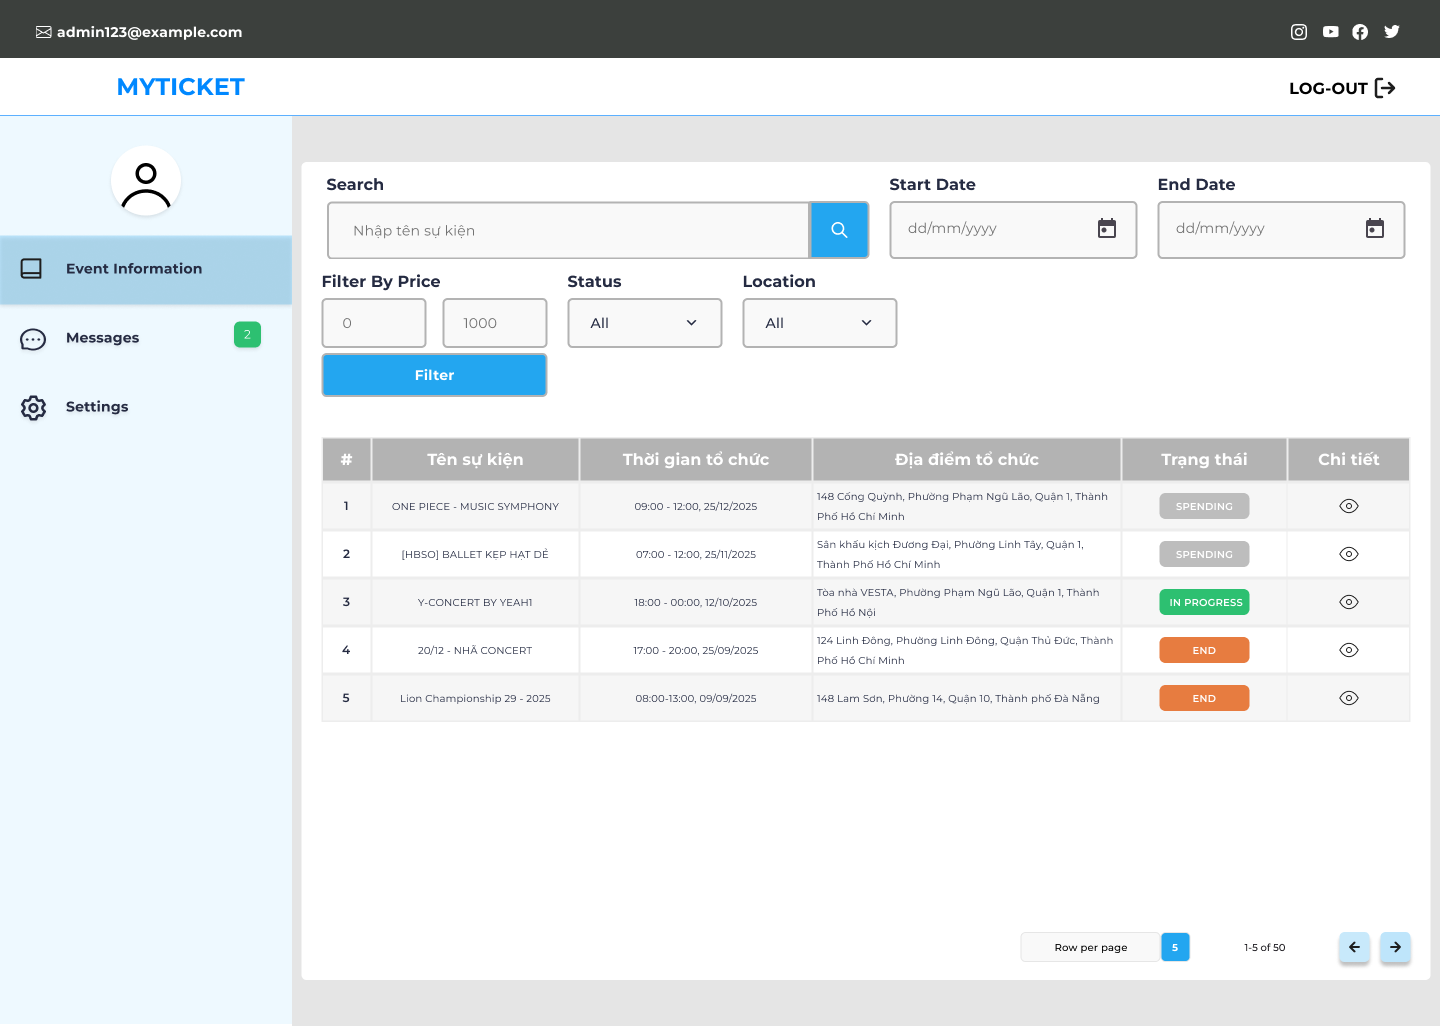
\includegraphics[width=0.75\textwidth]{Contents/UI/BTC/Ban tổ chức - Danh sách sự kiện (1).png}
    \vspace{15pt}
    \caption{Giao diện hiển thị danh sách các sự kiện của Ban tổ chức}
\end{figure}
\indent \indent Mô tả:\\
\indent - Sau khi xác thực tài khoản lúc đăng nhập, nếu role là Ban tổ chức thì hệ thống sẽ tự động điều hướng giao diện sang trang này.\\
\indent - Tại đây, Ban tổ chức có thể xem danh sách các sự kiện do mình tổ chức đã, đang và sẽ được đăng tải trên hệ thống.\\
\indent - Để tiện lợi cho việc xem thông tin sự kiện, Ban tổ chức có thể tìm kiếm bằng tên sự kiện hoặc lọc theo các tiêu chí sau:
\begin{itemize}
    \item[+] Start Date - End Start: thời gian tổ chức nằm trong phạm vị được chọn.
    \item[+] Filter By Price: tồn tại loại vé có giá nằm trong phạm vi được chọn.
    \item[+] Status: trạng thái bán vé bao gồm END (Đã kết thúc), IN PROCESS (Đang diễn ra) và SPENDING (Chuẩn bị)
    \item[+] Location: địa điểm tổ chức ở một tỉnh/thành phố cụ thể.
\end{itemize}
\indent - Ngoài ra, Ban tổ chức cũng có thể tùy chỉnh số hàng thông tin sự kiện sẽ hiển thị hoặc nhấn nút mũi tên để điều hướng.\\
\indent - Ban tổ chức có thể xem thêm thông tin chi tiết về các loại vé, giá bán vé, số lượng vé (ban đầu/đã bán/còn lại) cũng như lịch sử cập nhật trạng thái bán vé bằng cách di chuột vào con mắt ở cuối mỗi hàng thông tin sự kiện
\subsubsection{Chat giữa Ban tổ chức và người dùng}
\begin{figure}[H]
    \centering
    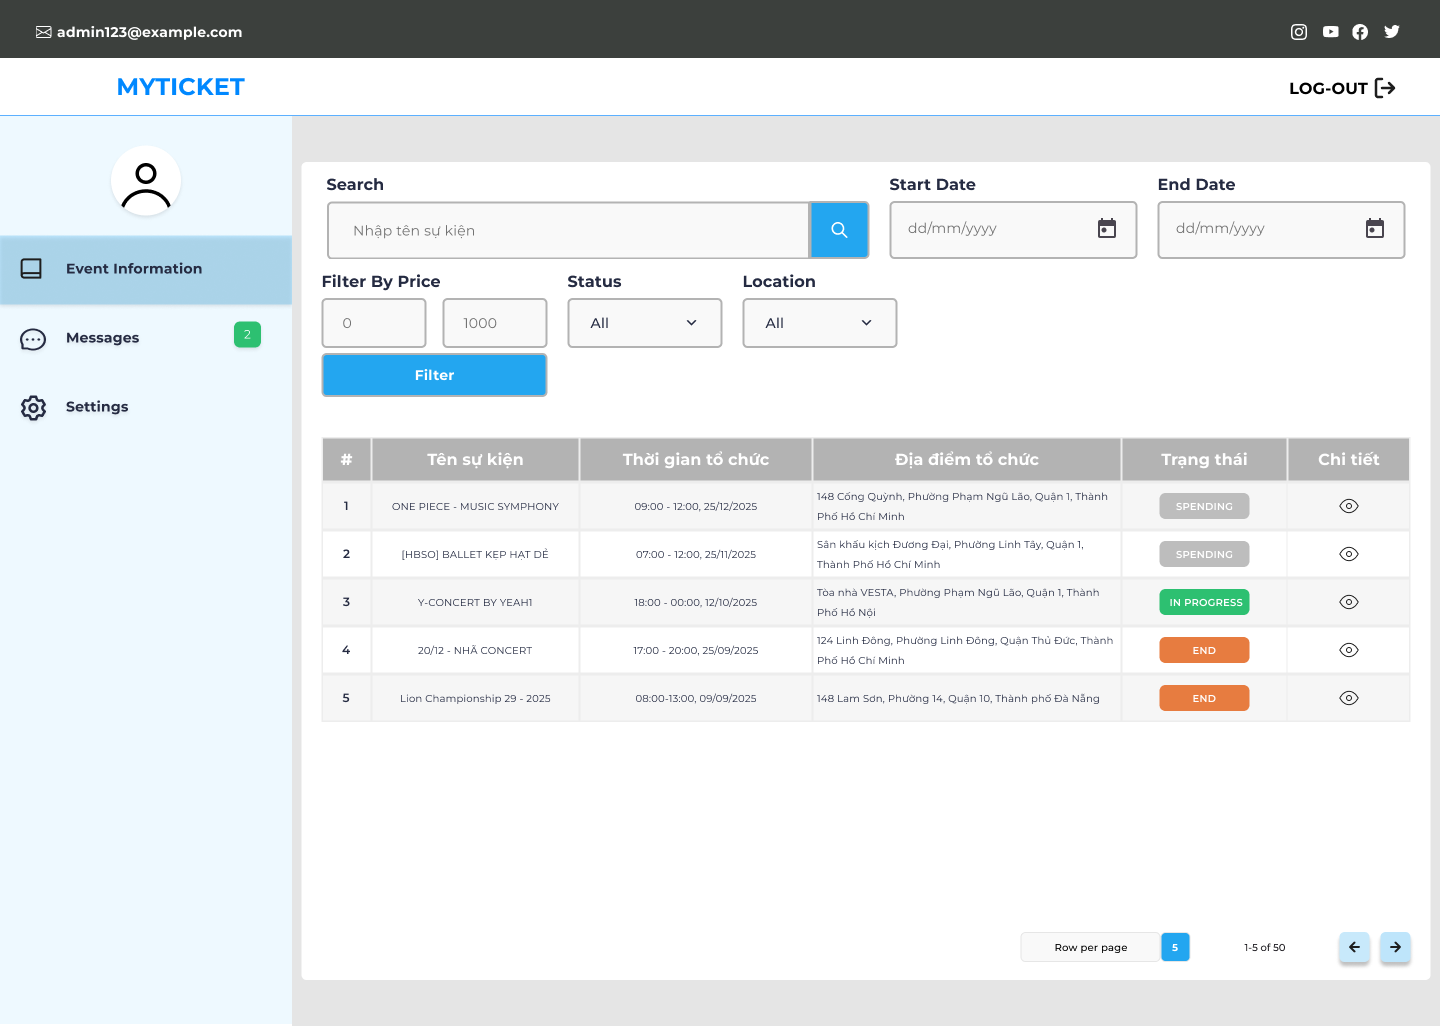
\includegraphics[width=0.75\textwidth]{Contents/UI/BTC/Ban tổ chức - Danh sách sự kiện (1).png}
    \vspace{15pt}
    \caption{Giao diện khung chat giữa Ban tổ chức và người dùng}
\end{figure}
\indent \indent Mô tả:
\indent - Số lượng tin nhắn chưa được đọc sẽ luôn được cập nhật tự động ở mục "Messages".\\
\indent - Tạo mục "Messages", Ban tổ chức sẽ được danh sách các người dùng có tin nhắn.\\
\indent - Các tin nhắn mới chưa đọc sẽ được hiển thị kèm dấu chấm xanh để tiện theo dõi. Khi được đọc, dấu chấm xanh sẽ tự động biến mất.\\
\indent - Sau khi Ban tổ chức chọn 1 người dùng cụ thể, hệ thống sẽ hiển thị giao diện khung chat cho phép phản hồi.
\subsection{Chức năng của Quản trị viên}
\subsubsection{Quản lý thông tin sự kiện}
\begin{figure}[H]
    \centering
    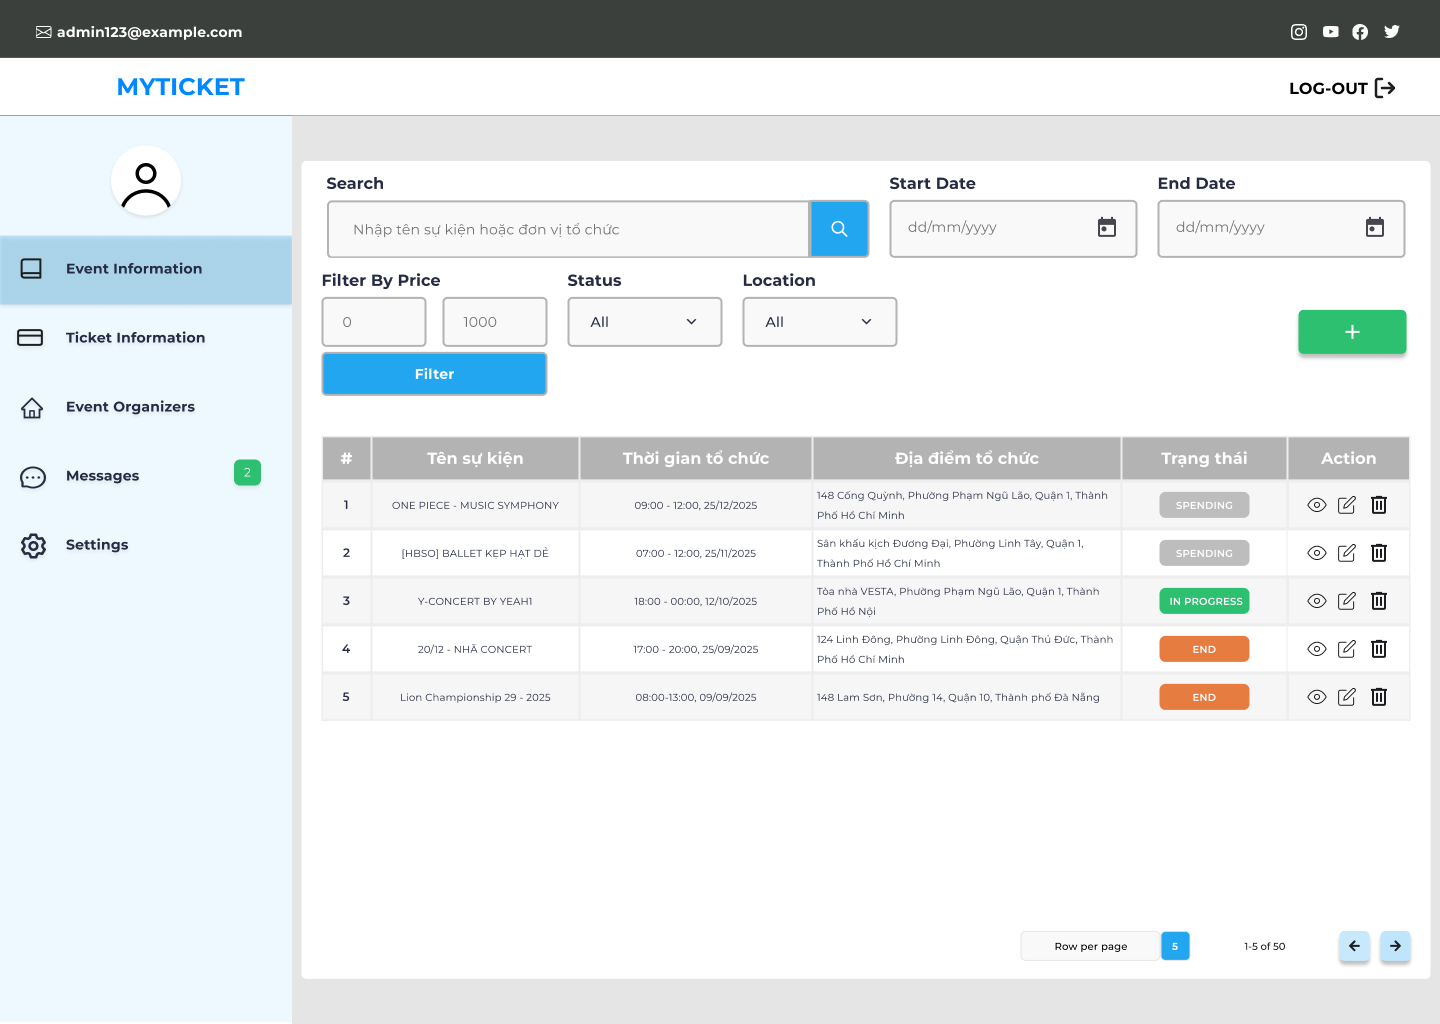
\includegraphics[width=0.75\textwidth]{Contents/UI/QTV/Quản trị viên - Danh sách sự kiện (1).png}
    \vspace{15pt}
    \caption{Giao diện quản lý thông tin sự kiện của Quản trị viên}
\end{figure}
\indent \indent Mô tả:\\
\indent - Sau khi xác thực tài khoản lúc đăng nhập, nếu role là Ban tổ chức thì hệ thống sẽ tự động điều hướng giao diện sang trang này.\\
\indent - Tại trang này, Quản trị viên có toàn quyền xem thông tin, chỉnh sửa thông tin, cập nhật trạng thái bán vé hoặc xóa một sự kiện cụ thể. \\
\indent - Quản trị viên cũng có thể sử dụng tính năng tìm kiếm sự kiến, lọc sự kiện hoặc sử dụng các tiện ích quan sát tương tự như ở phía Ban tổ chức.
\subsubsection{Tạo sự kiện mới}
\begin{figure}[H]
    \centering
    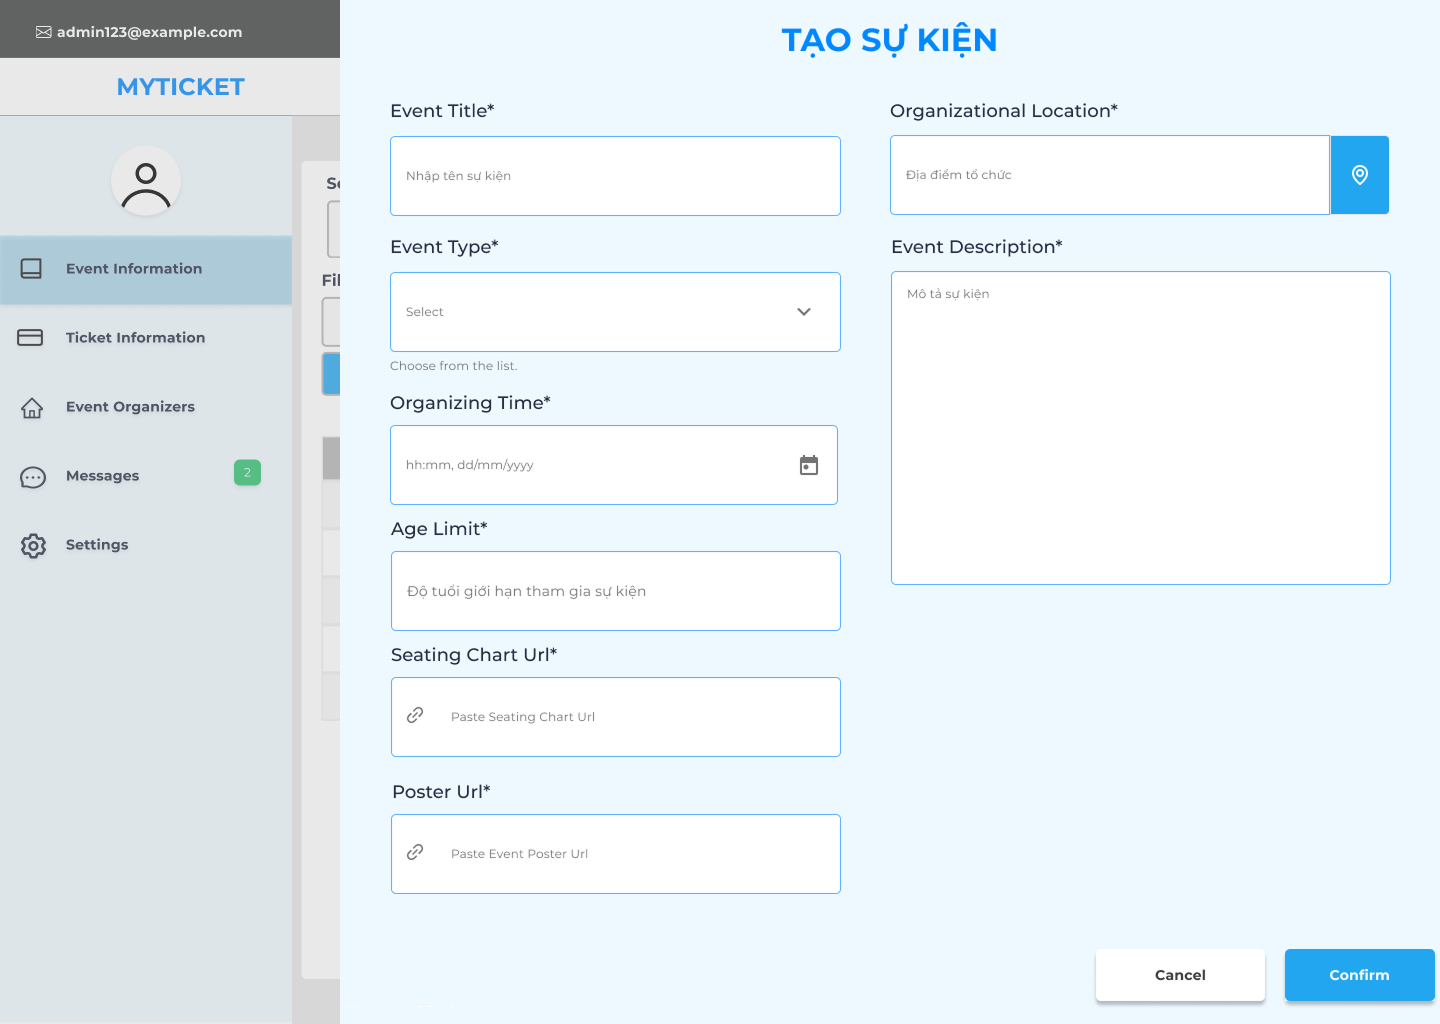
\includegraphics[width=0.75\textwidth]{Contents/UI/QTV/Quản trị viên - Tạo sự kiện (1).png}
    \vspace{15pt}
    \caption{Giao diện tạo sự kiện mới của Quản trị viên}
\end{figure}
\indent \indent Mô tả:\\
\indent - Quản trị viên là người có quyền thêm mới 1 sự kiện trong hệ thống bằng cách nhấn vào nút "+" ở trang Quản lý thông tin sự kiện. \\
\indent - Để tạo mới một sự kiện, Quản trị viên cần đảm bảo thông tin về Ban tổ chức của sự kiện này đã có trong hệ thống.

\subsubsection{Quản lý thông tin Ban tổ chức}
\begin{figure}[H]
    \centering
    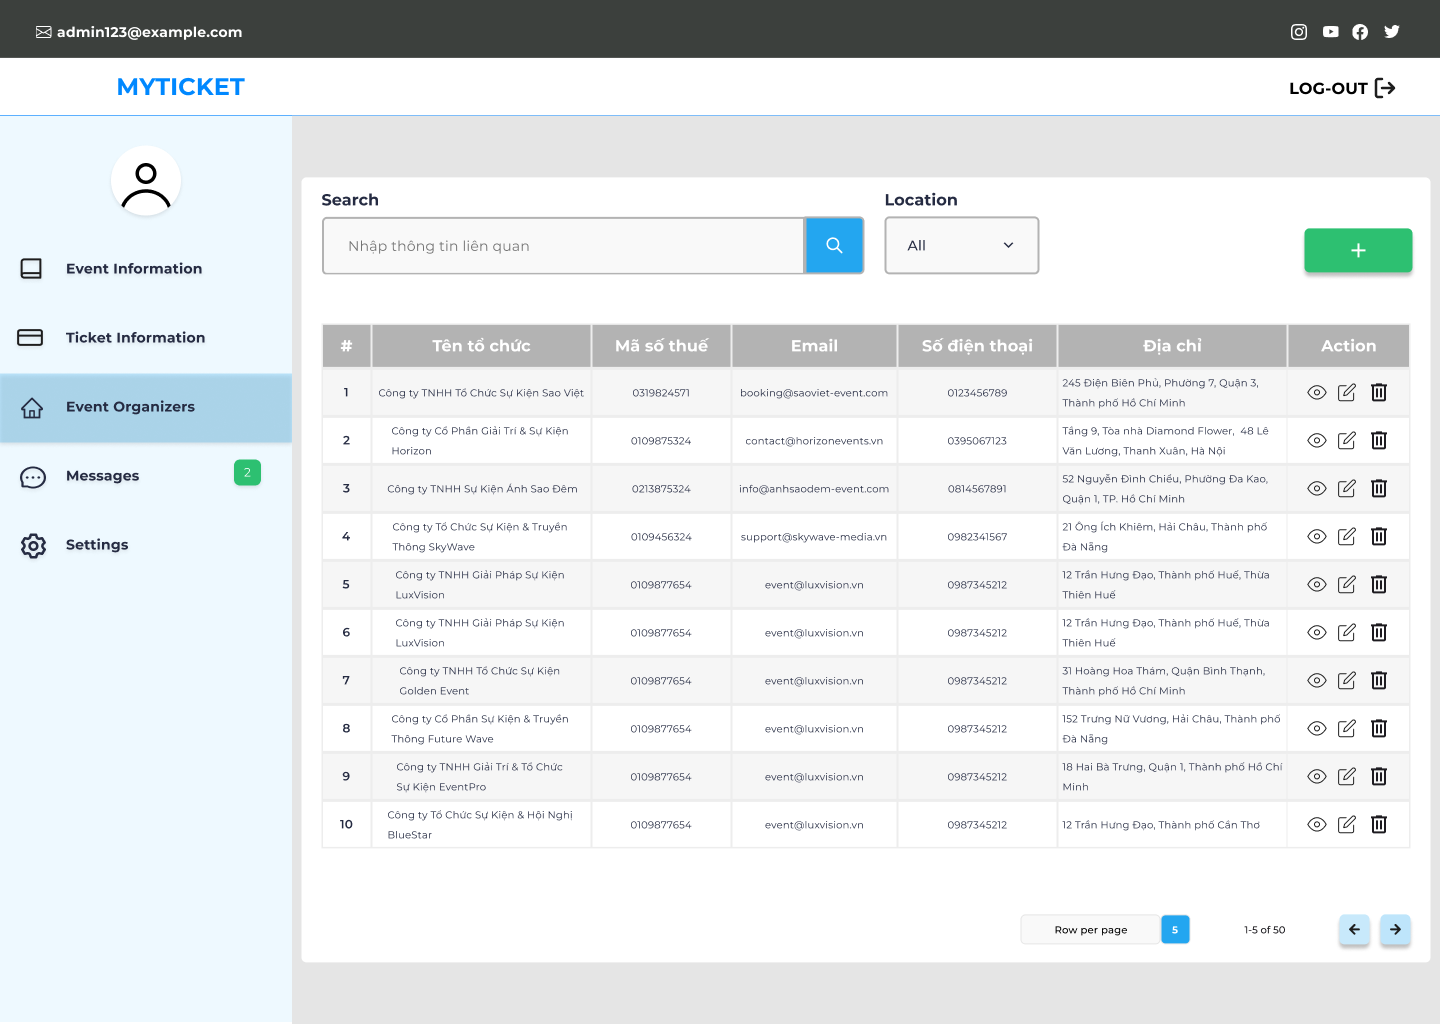
\includegraphics[width=0.75\textwidth]{Contents/UI/QTV/Quản trị viên - Danh sách đơn vị tổ chức sự kiện (1).png}
    \vspace{15pt}
    \caption{Giao diện quản lý thông tin Ban tổ chức của Quản trị viên}
\end{figure}
\indent \indent Mô tả: \\
\indent - Tại trang này, Quản trị viên có toàn quyền xem, chỉnh sửa hoặc xóa thông tin của một Ban tổ chức cụ thể.\\
\indent - Quản trị viên cũng có thể sử dụng chức năng tìm kiếm, lọc theo địa chỉ hoặc sử dụng các tiện ích để truy cập thông tin của những ban tổ chức dễ dàng hơn.

\subsubsection{Tạo ban tổ chức mới}
\begin{figure}[H]
    \centering
    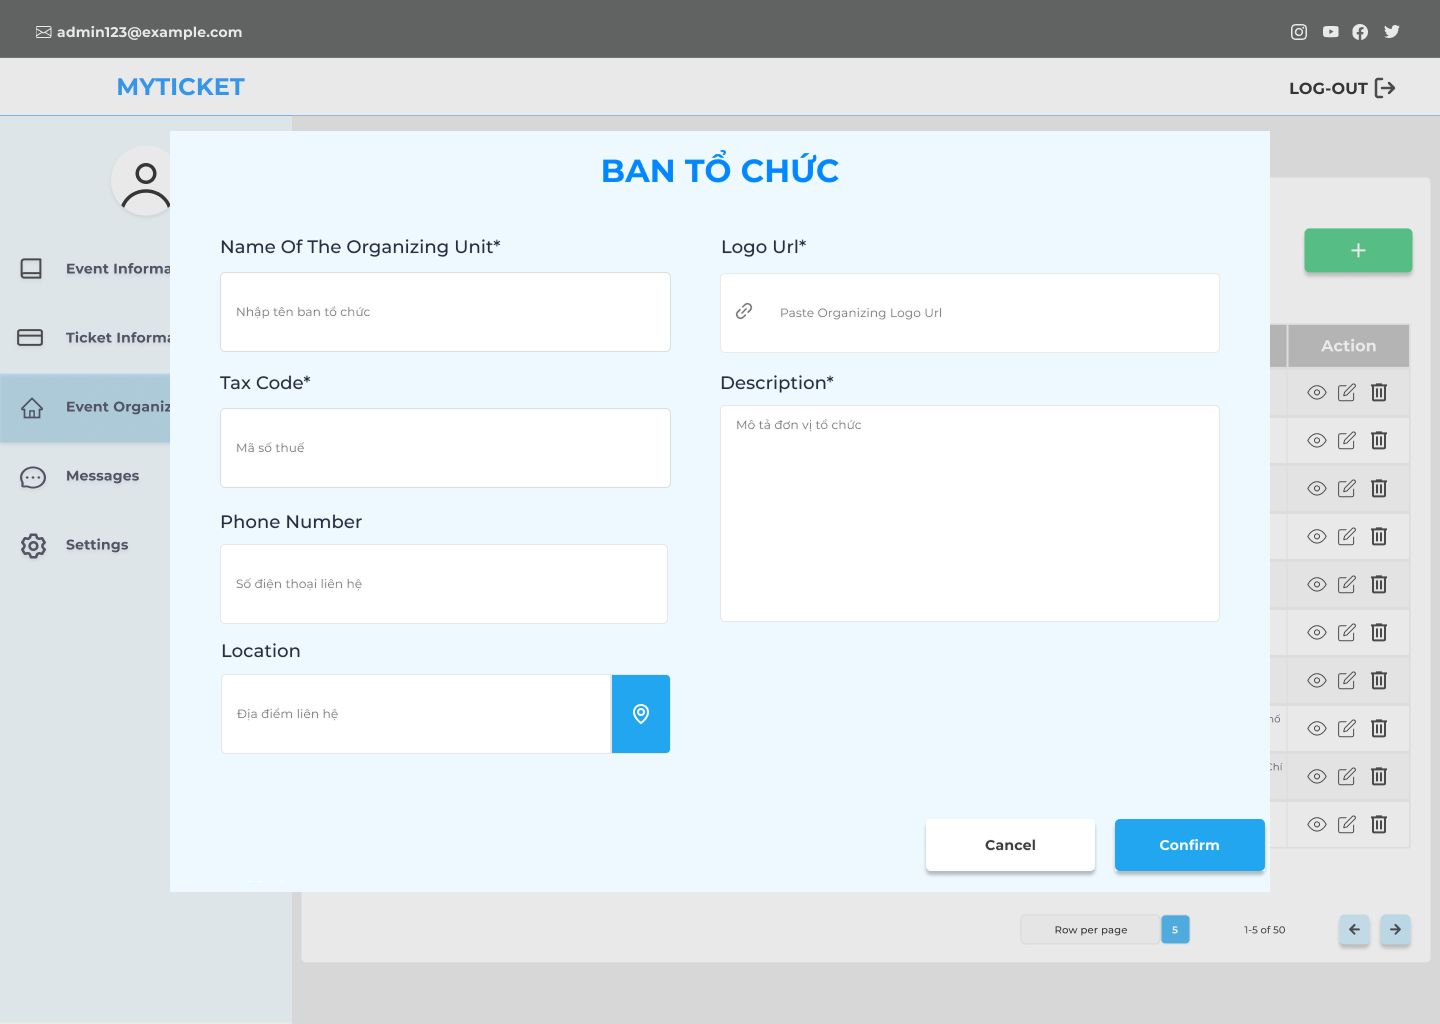
\includegraphics[width=0.75\textwidth]{Contents/UI/QTV/Quản trị viên - Thêm thông tin ban tổ chức.png}
    \vspace{15pt}
    \caption{Giao diện tạo ban tổ chức mới của Quản trị viên}
\end{figure}
\indent \indent Mô tả:\\
\indent - Quản trị viên là người có quyền thêm mới 1 Ban tổ chức trong hệ thống bằng cách nhấn vào nút "+" ở trang Quản lý thông tin Bản tổ chức. \\
\indent - Để tạo thành công, Quản trị viên bắt buộc phải điền đầy đủ thông tin ở các trường theo đúng format quy định.


\subsubsection{Thêm vé cho sự kiện}

\begin{figure}[H]
    \centering
    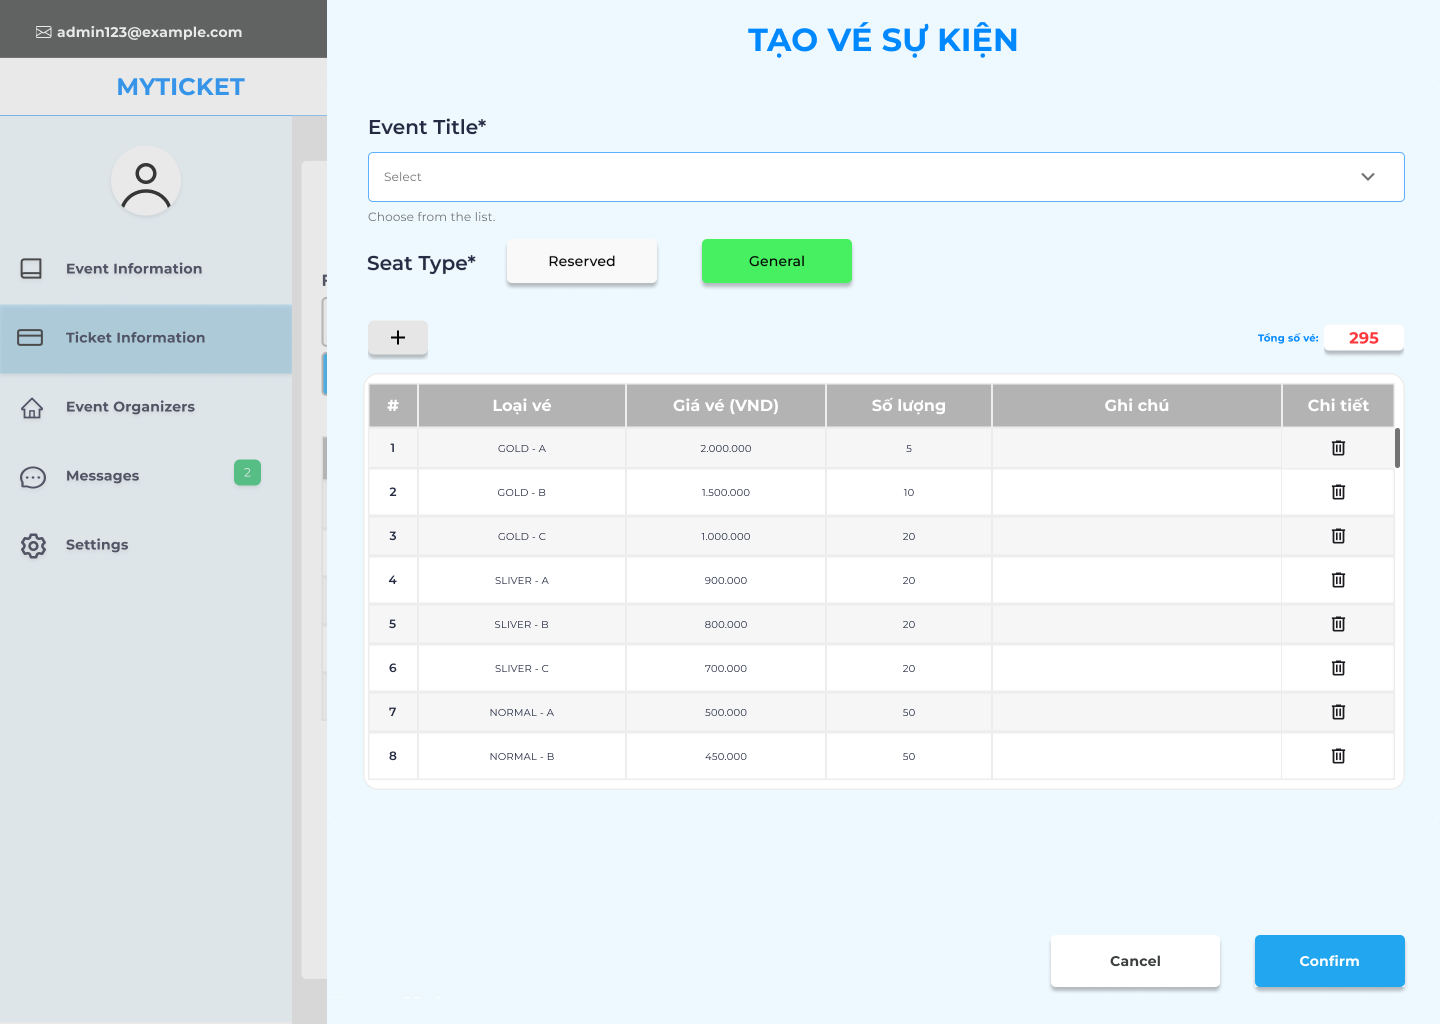
\includegraphics[width=0.75\textwidth]{Contents/UI/QTV/Quản trị viên - Tạo vé sự kiện (Vé không có chỗ ngồi cố định).png}
    \vspace{15pt}
    \caption{Giao diện tạo vé (loại vé không có chỗ ngồi cố định) cho sự kiện của Quản trị viên}
\end{figure}

\indent \indent Mô tả:\\
\indent - Quản trị viên chọn loại vé General và điền đầy đủ thông tin ở các trường theo đúng format quy định.

\begin{figure}[H]
    \centering
    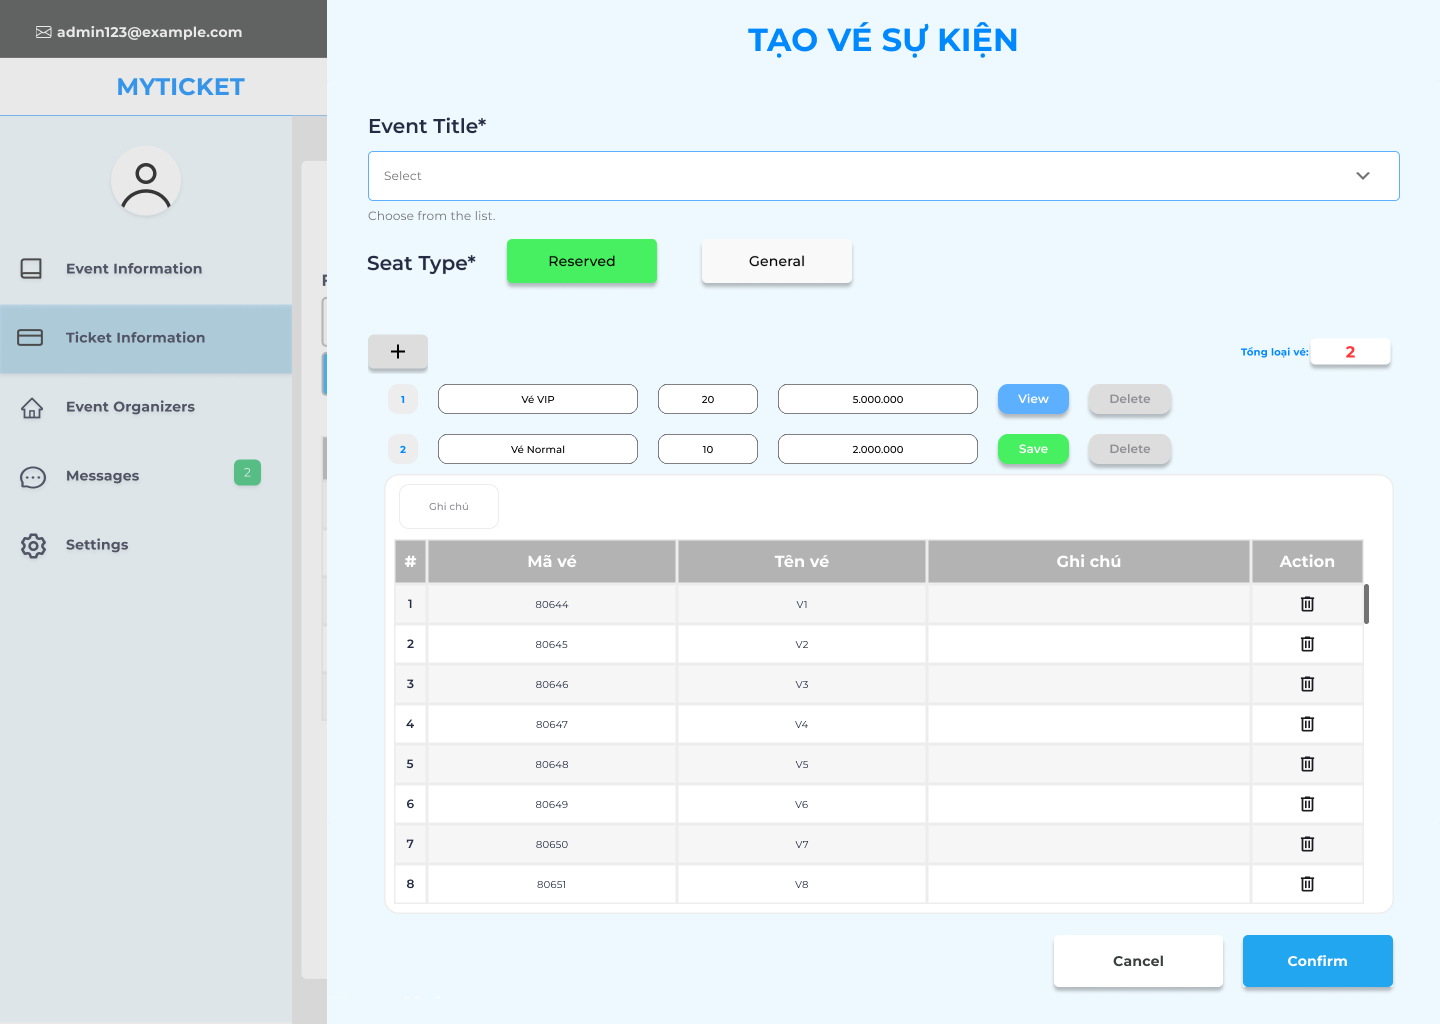
\includegraphics[width=0.75\textwidth]{Contents/UI/QTV/Quản trị viên - Tạo vé sự kiện (Vé có chỗ ngồi cố định).png}
    \vspace{15pt}
    \caption{Giao diện tạo vé (loại vé có chỗ ngồi cố định) cho sự kiện của Quản trị viên}
\end{figure}

\indent \indent Mô tả:\\
\indent \indent - Quản trị viên chọn loại vé Reserved, điền thông tin đầy đủ kèm theo tên và mã chỗ ngồi cố định.
